% ============================================================
%  IEEE Transactions on Power Systems  (or Power Delivery)
%  "Validation Boundaries of Reduced-Order Inverse Protection
%   Models Under Sixth-Order Synchronous Machine Dynamics"
%  Author: J. Eluvathingal
%  Build:  pdflatex × 3 + bibtex
% ============================================================
\documentclass[journal,twoside,letterpaper]{IEEEtran}

%% --- packages ---------------------------------------------------
\usepackage[T1]{fontenc}
\usepackage[utf8]{inputenc}
\usepackage{amsmath,amssymb,bm}
\usepackage{graphicx}
\usepackage{xcolor}
\usepackage{booktabs}
\usepackage{multirow}
\usepackage{cite}
\usepackage{url}
\usepackage{siunitx}
\usepackage{gensymb}
\usepackage{algorithm}
\usepackage{algpseudocode}
\usepackage{tikz}
\usepackage{pgfplots}
\pgfplotsset{compat=1.18}
\usetikzlibrary{positioning,shapes.geometric,shapes.misc,
                arrows.meta,chains,decorations.pathreplacing,
                calc,fit}
\usepgfplotslibrary{groupplots,fillbetween}

%% --- helpers ---------------------------------------------------
\newcommand{\vect}[1]{\bm{#1}}
\newcommand{\est}[1]{\hat{#1}}
\newcommand{\norm}[1]{\lVert#1\rVert}
\DeclareMathOperator{\clip}{clip}
\newtheorem{proposition}{Proposition}
\newtheorem{remark}{Remark}

%% =============================================================
\begin{document}

\title{Validation Boundaries of Reduced-Order Inverse Protection
       Models Under Sixth-Order Synchronous Machine Dynamics}

\author{Anoop~V.~Eluvathingal,~\IEEEmembership{Student Member,~IEEE,}
        and~K.~Shanti~Swarup,~\IEEEmembership{Senior Member,~IEEE}%
\thanks{Manuscript received \today.
        This work establishes the physics-faithful truth-model
        validation framework (Stage-2) for the SAMBP-SyncOC adaptive
        protection series and is part of the PhD research programme at
        the Department of Electrical Engineering, Indian Institute of
        Technology Madras, Chennai~600~036, India.}%
\thanks{A.~V.~Eluvathingal and K.~S.~Swarup are with the Department of
        Electrical Engineering, IIT Madras, Chennai~600~036, India
        (e-mail: ee21d017@smail.iitm.ac.in; swarup@ee.iitm.ac.in).}}

\markboth{IEEE Transactions on Power Systems,~Vol.~XX,
No.~X, \MakeUppercase{Month}~2026}%
{Eluvathingal \& Swarup: Validation Boundaries of Reduced-Order Inverse
Protection Models}

\maketitle

%% =============================================================
\begin{abstract}
Reduced-order inverse models are attractive for real-time
adaptive overcurrent protection because they identify
relay-relevant source parameters within a protection operating
interval.
Their reliability, however, depends on the degree to which the
true generator fault response remains representable by the
reduced waveform model over the estimation window.
This paper develops a physics-faithful forward benchmark based
on a sixth-order synchronous-machine Park~$dq$ model with
automatic voltage regulator (AVR), power system stabilizer
(PSS), and governor dynamics, and uses it to quantify the
validity limits of the Stage-1 reduced-order inverse protection
model.
The forward benchmark is formulated as a nine-state stiff
ordinary differential equation (ODE) system, coupled to a
stator algebraic interface and inverse Park transformation to
generate relay-observable three-phase currents.
Window-dependent model mismatch is evaluated using four
complementary metrics: waveform residual norm, parameter bias,
normalised Jacobian condition number, and confidence-gate
behaviour.
Results show that the reduced model remains relay-valid for
estimation windows up to approximately~150~ms, achieving
waveform residuals below~0.05~p.u.\ and confidence scores
above the acceptance threshold~$\gamma_{th}=0.70$.
Beyond this boundary, AVR-driven evolution of the sustained
current component progressively biases the estimated
steady-state current~$\hat{I}_{ss}$ downward and inflates the
estimated AC time constant~$\hat{\tau}_{ac}$, causing pickup
errors exceeding 10\% and trip-time deviations exceeding
the grading margin requirement.
A relay-validity map is presented that delineates the
window-length and operating-point region over which reduced
inverse adaptation may be trusted, cautioned, or blocked.
The paper thus provides a protection-oriented
identifiability and fidelity framework for the deployment of
reduced inverse estimators in adaptive relay IEDs.
\end{abstract}

\begin{IEEEkeywords}
adaptive overcurrent protection, synchronous generator,
Park $dq$ model, sixth-order machine model, inverse estimation,
window validity, Levenberg--Marquardt, condition number,
confidence gate, AVR, PSS, governor.
\end{IEEEkeywords}

%% =============================================================
\section{Introduction}
\label{sec:intro}

\subsection{Motivation}

Online parameter estimation offers a principled route to
adaptive overcurrent protection: rather than selecting from a
discrete table of pre-computed settings, the relay fits a
parametric fault-current model to the observed waveform and
maps the result directly to protective relay settings
\cite{Eluvathingal2025_TR01,Lazkano2000}.
The Stage-1 SAMBP-SyncOC framework demonstrated that a
six-parameter reduced inverse model, fitted by a two-pass
Levenberg--Marquardt (LM) estimator, can extract relay-relevant
quantities within the first few cycles after fault
inception~\cite{Eluvathingal2025_TR01}.

The reduced model captures the dominant waveform features:
an AC transient driven by the direct-axis transient time
constant, a DC offset decaying with the armature circuit time
constant, and a steady-state sinusoidal component whose
magnitude approximates the post-fault rms current.
These features are fully present within the first 100--150~ms
of a fault.

Over longer windows, however, the true generator response is
shaped by controller dynamics that the reduced model
deliberately omits:
\begin{itemize}
  \item The AVR boosts field voltage $E_{fd}$ within
    $\sim$0.1~s, causing the sustained current $I_{ss}$ to
    rise progressively after the initial subtransient period.
  \item The governor adjusts mechanical torque $T_m$ on a
    $\sim$0.5~s time scale, modifying the air-gap torque
    balance and rotor speed.
  \item The PSS injects a damping signal into the AVR to
    suppress rotor oscillations, creating superimposed
    oscillatory components in the fault current.
\end{itemize}
None of these dynamics appear in the six-parameter reduced
model.
When the estimation window extends into the range where these
dynamics are active, the reduced model is mis-specified: the
LM estimator minimises residuals by distorting the inferred
parameters, introducing systematic bias that may degrade relay
decisions.

\subsection{Gap in the literature}

Prior work on adaptive overcurrent protection addresses
estimator design~\cite{Lazkano2000,Sachdev1985} or relay
logic~\cite{Urdaneta1988,So2000}, but rarely asks the
foundational question: \emph{over what window is the reduced
model a sufficiently faithful representation of the true fault
current for adaptive relay decisions}?

Physics-based synchronous-machine models of the sixth-order
Park~$dq$ form are well-established in power system
stability analysis~\cite{Kundur1994,Anderson1977}.
They have not, however, been systematically employed as
truth-model benchmarks for evaluating relay-relevant
identifiability boundaries.
This paper bridges that gap.

\subsection{Paper objective}

The central objective is to \emph{quantify the relay-validity
boundary of the reduced inverse protection model under
sixth-order synchronous-machine dynamics with AVR, PSS, and
governor}.
The sixth-order model is not proposed as an alternative
estimator --- it is computationally prohibitive for real-time
IED use --- but as a physics-faithful ground truth against
which the simpler model's accuracy is measured.
Fig.~\ref{fig:concept} illustrates the three-layer
architecture of this study.

\begin{figure}[!t]
  \centering
  % ============================================================
%  Figure 1 — Paper concept: three-layer framework
%  Layer 1: Sixth-Order Truth Model
%  Layer 2: Reduced Inverse Estimator
%  Layer 3: Relay Decision / Confidence Gate
% ============================================================
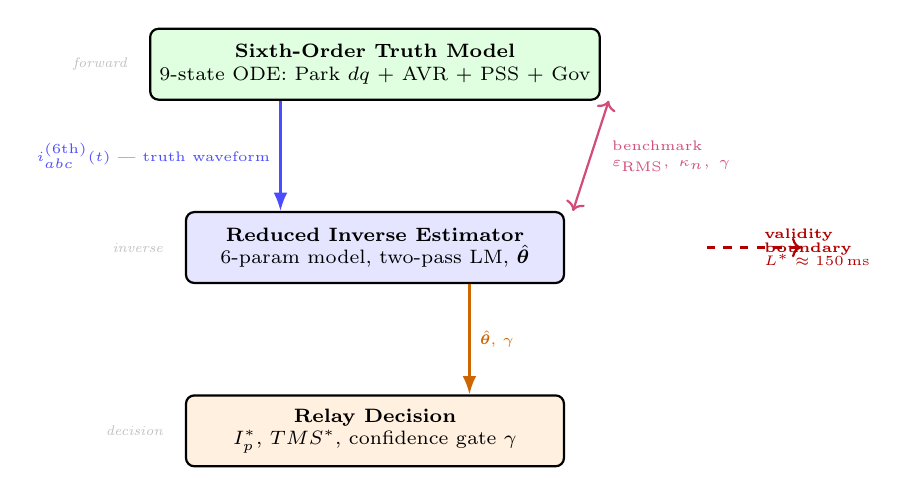
\begin{tikzpicture}[
  every node/.style={font=\scriptsize},
  proc/.style={draw, thick, rounded corners=3pt,
               minimum width=4.8cm, minimum height=0.90cm,
               align=center},
  arr/.style={->, thick, >=Latex},
  node distance=1.4cm
]

%% --- Layers ---------------------------------------------------
\node[proc, fill=green!12]  (truth)
     {\textbf{Sixth-Order Truth Model} \\
      9-state ODE: Park $dq$ + AVR + PSS + Gov};

\node[proc, fill=blue!10, below=of truth]  (estim)
     {\textbf{Reduced Inverse Estimator} \\
      6-param model, two-pass LM, $\hat{\bm\theta}$};

\node[proc, fill=orange!12, below=of estim] (relay)
     {\textbf{Relay Decision} \\
      $I_p^*$, $TMS^*$, confidence gate $\gamma$};

%% --- Left: truth waveform arrow ------------------------------
\draw[arr, blue!70]
  ([xshift=-1.2cm]truth.south) --
  node[left, font=\tiny, blue!70]
  {$i_{abc}^{(6\text{th})}(t)$ --- truth waveform}
  ([xshift=-1.2cm]estim.north);

%% --- Right: parameter arrow ----------------------------------
\draw[arr, orange!80!black]
  ([xshift=1.2cm]estim.south) --
  node[right, font=\tiny, orange!80!black]
  {$\hat{\bm\theta}$, $\gamma$}
  ([xshift=1.2cm]relay.north);

%% --- Middle: benchmark comparison bracket --------------------
\draw[<->, thick, purple!70]
  ([xshift=0.1cm]truth.south east) --
  ([xshift=0.1cm]estim.north east)
  node[midway, right=4pt, align=left, font=\tiny, purple!70]
  {benchmark\\$\varepsilon_{\mathrm{RMS}},\;\kappa_n,\;\gamma$};

%% --- Validity boundary annotation ---------------------------
\draw[->, thick, red!70!black, dashed]
  ([xshift=1.8cm]estim.east) --
  node[right, font=\tiny, red!70!black, align=left]
  {\textbf{validity}\\[-0.5ex]\textbf{boundary}\\[-0.5ex]$L^\ast \approx 150$\,ms}
  ++(1.2, 0);

%% --- Vertical arrow labels on left side of nodes ------------
\node[font=\tiny, gray!50, left=4pt] at (truth.west)
     {\textit{forward}};
\node[font=\tiny, gray!50, left=4pt] at (estim.west)
     {\textit{inverse}};
\node[font=\tiny, gray!50, left=4pt] at (relay.west)
     {\textit{decision}};

\end{tikzpicture}

  \caption{Paper framework: the sixth-order truth model
    generates relay-observable fault currents that benchmark
    the reduced inverse estimator.
    The validity boundary defines where the estimator remains
    accurate enough for adaptive relay decisions.}
  \label{fig:concept}
\end{figure}

\subsection{Contributions}

The main contributions are as follows.
\begin{enumerate}
  \item A physics-faithful sixth-order Park~$dq$ forward
    benchmark for synchronous-generator fault-current
    simulation, augmented with AVR, PSS, and governor
    dynamics, coupled to a stator algebraic interface and
    inverse Park transformation to generate relay-observable
    abc currents (Section~\ref{sec:sixthorder}).
  \item A protection-oriented validation methodology
    comparing the reduced inverse model against the
    sixth-order benchmark across window lengths, fault types,
    and operating conditions, using four
    relay-relevant metrics (Section~\ref{sec:methodology}).
  \item A window-validity analysis identifying the time
    horizon up to which the reduced inverse model is relay
    valid ($L^\ast \approx 150$~ms), and beyond which
    neglected AVR/PSS/governor dynamics materially bias
    estimated parameters (Section~\ref{sec:results}).
  \item An identifiability and confidence study linking
    residual growth to Jacobian conditioning, parameter bias,
    and confidence-gate behaviour in the Stage-1 inverse
    estimator (Section~\ref{sec:results}).
  \item A relay-validity map and practical deployment
    guidelines specifying when reduced inverse adaptation
    may be trusted, flagged, or blocked
    (Sections~\ref{sec:results} and~\ref{sec:discussion}).
\end{enumerate}

%% =============================================================
\section{Baseline Reduced-Order Inverse Protection Model}
\label{sec:baseline}

\subsection{Analytical waveform model}

The Stage-1 reduced inverse model represents the phase-A
fault current as~\cite{Eluvathingal2025_TR01}
\begin{equation}
  i_a^{(1)}(t) = \bigl[I_{ss} + (I_{sub} - I_{ss})\,
                  e^{-t_{\mathrm{rel}}/\tau_{ac}}\bigr]
                  \sin(\omega t + \varphi_a)
                - I_{sub}\sin(\varphi_a)\,
                  e^{-t_{\mathrm{rel}}/\tau_{dc}},
  \quad t \geq t_0,
\label{eq:reduced_model}
\end{equation}
where $t_{\mathrm{rel}} = t - t_0$, $I_{ss}$ is the sustained
(steady-state) current magnitude, $I_{sub}$ is the subtransient
peak, $\tau_{ac}$ is the AC decay time constant (approximately
$T'_{d0}$), $\tau_{dc}$ is the DC offset decay constant, and
$\varphi_a$ is the fault inception angle for phase~A.
The term $-I_{sub}\sin(\varphi_a)\,e^{-t/\tau_{dc}}$ provides
the maximum possible DC offset consistent with
$i_a(t_0) = 0$~\cite{Anderson1977}.

The six-parameter vector is
\begin{equation}
  \vect\theta = \bigl[t_0,\;I_{ss},\;I_{sub},\;
                      \tau_{ac},\;\tau_{dc},\;\varphi_a\bigr]^\top.
\label{eq:theta}
\end{equation}

\subsection{Two-pass Levenberg--Marquardt estimator}

Pass~1 seeds $I_{ss}$ from the pre-fault rms current and
minimises
\begin{equation}
  \hat{\vect\theta}^{(1)} = \arg\min_{\vect\theta}\;
    \sum_{n \in \mathcal{W}}\bigl[i_a(t_n) -
    i_a^{(1)}(\vect\theta, t_n)\bigr]^2,
\label{eq:lm}
\end{equation}
over window $\mathcal{W} = \{t_n : t_0 \leq t_n \leq t_0+L\}$.
Pass~2 uses $\hat{\vect\theta}^{(1)}$ as a warm start and
refines the estimate.
Fig.~\ref{fig:estimator_recap} shows the estimator
architecture.

\begin{figure}[!t]
  \centering
  % ============================================================
%  Figure 2 — Stage-1 reduced inverse estimator flowchart
% ============================================================
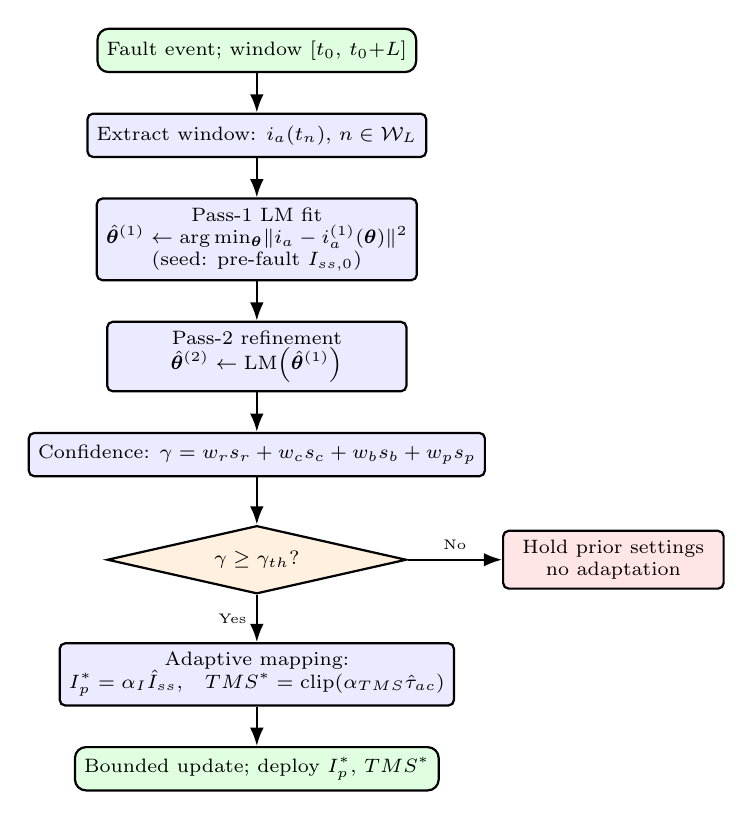
\begin{tikzpicture}[
  every node/.style={font=\scriptsize},
  proc/.style ={draw, thick, fill=blue!8, rounded corners=2pt,
                minimum width=3.8cm, minimum height=0.55cm,
                align=center},
  dec/.style  ={draw, thick, fill=orange!12, diamond, aspect=3.2,
                minimum width=3.8cm, align=center},
  term/.style ={draw, thick, fill=green!12, rounded corners=4pt,
                minimum width=3.8cm, minimum height=0.55cm,
                align=center},
  warn/.style ={draw, thick, fill=red!10, rounded corners=2pt,
                minimum width=2.8cm, minimum height=0.55cm,
                align=center},
  arr/.style  ={->, thick, >=Latex},
  node distance=0.50cm
]

\node[term]  (start)  {Fault event; window $[t_0,\,t_0{+}L]$};

\node[proc, below=of start] (extract)
     {Extract window: $i_a(t_n)$, $n \in \mathcal{W}_L$};

\node[proc, below=of extract] (pass1)
     {Pass-1 LM fit\\
      $\hat{\bm\theta}^{(1)} \leftarrow
       \arg\min_{\bm\theta}\norm{i_a - i_a^{(1)}(\bm\theta)}^2$\\
      (seed: pre-fault $I_{ss,0}$)};

\node[proc, below=of pass1] (pass2)
     {Pass-2 refinement\\
      $\hat{\bm\theta}^{(2)} \leftarrow
       \mathrm{LM}\!\left(\hat{\bm\theta}^{(1)}\right)$};

\node[proc, below=of pass2] (conf)
     {Confidence: $\gamma = w_r s_r + w_c s_c + w_b s_b + w_p s_p$};

\node[dec, below=0.6 of conf] (gate) {$\gamma \geq \gamma_{th}$?};

\node[warn, right=1.2 of gate] (hold)
     {Hold prior settings\\no adaptation};
\draw[arr] (gate) -- node[above,font=\tiny]{No} (hold);

\node[proc, below=0.6 of gate] (map)
     {Adaptive mapping:\\
      $I_p^* = \alpha_I\hat{I}_{ss}$,\quad
      $TMS^* = \mathrm{clip}(\alpha_{TMS}\hat\tau_{ac})$};

\node[term, below=of map] (deploy)
     {Bounded update; deploy $I_p^*$, $TMS^*$};

\draw[arr] (start) -- (extract);
\draw[arr] (extract) -- (pass1);
\draw[arr] (pass1) -- (pass2);
\draw[arr] (pass2) -- (conf);
\draw[arr] (conf) -- (gate);
\draw[arr] (gate) -- node[left,font=\tiny]{Yes} (map);
\draw[arr] (map) -- (deploy);

\end{tikzpicture}

  \caption{Stage-1 reduced inverse estimator: two-pass
    Levenberg--Marquardt fit followed by confidence gating
    and adaptive relay mapping.}
  \label{fig:estimator_recap}
\end{figure}

\subsection{Confidence gate and adaptive mapping}

The scalar confidence score is computed as
\begin{equation}
  \gamma = w_r\,s_r + w_c\,s_c + w_b\,s_b + w_p\,s_p,
\label{eq:confidence}
\end{equation}
where $s_r$ is a normalised residual score, $s_c$ is a
condition-number score, $s_b$ is a bound-proximity score,
and $s_p$ is a prior-consistency score~\cite{Eluvathingal2025_TR01}.
Adaptation proceeds only if $\gamma \geq \gamma_{th} = 0.70$.

When accepted, the relay settings are updated as
\begin{align}
  I_p^\ast &= \alpha_I\,\hat{I}_{ss},  \label{eq:ip_adapt}\\
  TMS^\ast &= \clip\!\bigl(\alpha_{TMS}\,\hat\tau_{ac},\;
               TMS_{\min},\;TMS_{\max}\bigr), \label{eq:tms_adapt}
\end{align}
with bounded incremental update
\begin{align}
  \Delta I_p &= \clip\!\bigl(I_p^\ast - I_{p,\mathrm{cur}},\;
                [-\delta,+\delta]\bigr),\label{eq:bounded_a}\\
  I_{p,\mathrm{final}} &= \clip\!\bigl(I_{p,\mathrm{cur}} + \Delta I_p,\;
                [I_p^{\min},\;I_p^{\max}]\bigr).\label{eq:bounded_b}
\end{align}
This bounded update law prevents single-event runaway
adaptation~\cite{Eluvathingal2025_TR01}.

Table~\ref{tab:baseline_params} summarises the baseline
reduced-model parameters used in this study.

\begin{table}[!t]
\caption{Baseline reduced inverse model: parameters and
         estimation outputs (3PH fault, nominal operating point)}
\label{tab:baseline_params}
\centering
\renewcommand{\arraystretch}{1.15}
\begin{tabular}{lcc}
\toprule
Parameter & Symbol & Nominal value \\
\midrule
Steady-state current      & $I_{ss}$      & 1.35~p.u. \\
Subtransient current      & $I_{sub}$     & 3.20~p.u. \\
AC decay constant         & $\tau_{ac}$   & 0.83~s \\
DC offset constant        & $\tau_{dc}$   & 0.07~s \\
Fault inception angle     & $\varphi_a$   & $-30\degree$ \\
Pickup scaling            & $\alpha_I$    & 0.80 \\
TMS scaling               & $\alpha_{TMS}$& 0.12 \\
Confidence threshold      & $\gamma_{th}$ & 0.70 \\
Bounded step              & $\delta$      & 0.10~p.u. \\
\bottomrule
\end{tabular}
\end{table}

%% =============================================================
\section{Sixth-Order Park \boldmath{$dq$} Forward Truth Model}
\label{sec:sixthorder}

\subsection{Model overview}

The sixth-order model is the \emph{forward truth benchmark}.
It simulates the physical generator fault response including
all significant electromechanical and controller dynamics,
and produces relay-observable abc currents that serve as the
ground truth against which the reduced inverse model is
evaluated.
It is emphatically not used online in the relay: its
nine-state stiff ODE system and Radau integration are
computationally unsuitable for IED-grade real-time use.

Fig.~\ref{fig:sixthorder_model} shows the complete block
structure.

\begin{figure}[!t]
  \centering
  % ============================================================
%  Figure 3 — Sixth-order Park dq truth model block diagram
% ============================================================
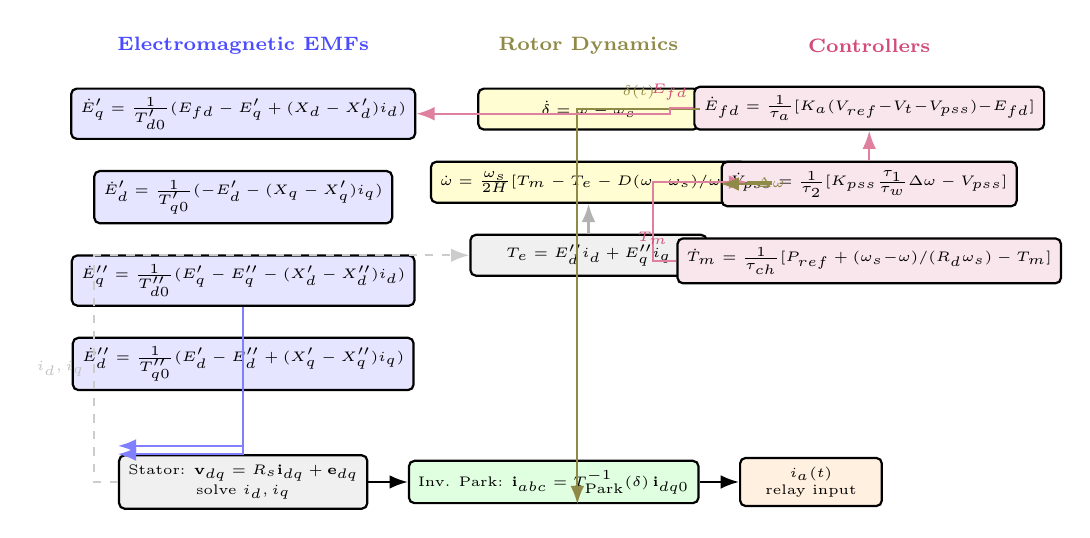
\begin{tikzpicture}[
  every node/.style={font=\tiny},
  emf/.style  ={draw, thick, fill=blue!10, rounded corners=2pt,
                minimum width=2.8cm, minimum height=0.52cm,
                align=center},
  swing/.style={draw, thick, fill=yellow!18, rounded corners=2pt,
                minimum width=2.8cm, minimum height=0.52cm,
                align=center},
  ctrl/.style ={draw, thick, fill=purple!10, rounded corners=2pt,
                minimum width=2.8cm, minimum height=0.52cm,
                align=center},
  iface/.style={draw, thick, fill=gray!12, rounded corners=2pt,
                minimum width=3.0cm, minimum height=0.52cm,
                align=center},
  park/.style ={draw, thick, fill=green!12, rounded corners=2pt,
                minimum width=3.0cm, minimum height=0.52cm,
                align=center},
  arr/.style  ={->, thick, >=Latex},
  node distance=0.38cm
]

%% --- Column headers ------------------------------------------
\node[font=\scriptsize\bfseries, blue!70] (hdr_emf) at (0, 0)
     {Electromagnetic EMFs};
\node[font=\scriptsize\bfseries, yellow!50!black, right=1.4cm of hdr_emf] (hdr_sw)
     {Rotor Dynamics};
\node[font=\scriptsize\bfseries, purple!70, right=1.4cm of hdr_sw] (hdr_ctrl)
     {Controllers};

%% --- EMF column (left) ---------------------------------------
\node[emf, below=0.3 of hdr_emf] (Eqp)
     {$\dot{E}'_q = \tfrac{1}{T'_{d0}}(E_{fd}-E'_q+(X_d-X'_d)i_d)$};
\node[emf, below=of Eqp] (Edp)
     {$\dot{E}'_d = \tfrac{1}{T'_{q0}}(-E'_d-(X_q-X'_q)i_q)$};
\node[emf, below=of Edp] (Eqpp)
     {$\dot{E}''_q = \tfrac{1}{T''_{d0}}(E'_q-E''_q-(X'_d-X''_d)i_d)$};
\node[emf, below=of Eqpp] (Edpp)
     {$\dot{E}''_d = \tfrac{1}{T''_{q0}}(E'_d-E''_d+(X'_q-X''_q)i_q)$};

%% --- Rotor column (middle) -----------------------------------
\node[swing, below=0.3 of hdr_sw] (delta)
     {$\dot\delta = \omega - \omega_s$};
\node[swing, below=of delta] (omega)
     {$\dot\omega = \frac{\omega_s}{2H}[T_m - T_e - D(\omega{-}\omega_s)/\omega_s]$};
\node[iface, below=of omega] (Te)
     {$T_e = E''_d i_d + E''_q i_q$};

%% --- Controller column (right) -------------------------------
\node[ctrl, below=0.3 of hdr_ctrl] (avr)
     {$\dot{E}_{fd} = \tfrac{1}{\tau_a}[K_a(V_{ref}{-}V_t{-}V_{pss}){-}E_{fd}]$};
\node[ctrl, below=of avr] (pss)
     {$\dot{V}_{pss} = \tfrac{1}{\tau_2}[K_{pss}\tfrac{\tau_1}{\tau_w}\Delta\omega - V_{pss}]$};
\node[ctrl, below=of pss] (gov)
     {$\dot{T}_m = \tfrac{1}{\tau_{ch}}[P_{ref} + (\omega_s{-}\omega)/(R_d\omega_s) - T_m]$};

%% --- Bottom row: stator interface and Park transform ---------
\node[iface, below=0.8 of Edpp]  (stator)
     {Stator: $\mathbf{v}_{dq} = R_s\mathbf{i}_{dq} + \mathbf{e}_{dq}$\\ solve $i_d, i_q$};
\node[park,  right=0.5cm of stator] (parkinv)
     {Inv. Park: $\mathbf{i}_{abc} = T^{-1}_{\mathrm{Park}}(\delta)\,\mathbf{i}_{dq0}$};
\node[draw, thick, fill=orange!12, rounded corners=2pt,
      minimum width=1.8cm, minimum height=0.52cm, align=center,
      right=0.5cm of parkinv] (output)
     {$i_a(t)$\\relay input};

%% --- Key arrows ----------------------------------------------
% E'' → stator
\draw[arr, blue!50] (Eqpp.south) |- (stator.north west);
\draw[arr, blue!50] (Edpp.south) |- ([yshift=3pt]stator.north west);
% stator → Park
\draw[arr] (stator.east) -- (parkinv.west);
\draw[arr] (parkinv.east) -- (output.west);
% δ → Park
\draw[arr, yellow!50!black] (delta.east) -| ([xshift=0.3cm]parkinv.south)
     node[near start, above, font=\tiny] {$\delta(t)$};
% T_e → ω
\draw[arr, gray!60] (Te.north) -- (omega.south);
% E_fd → E'_q
\draw[arr, purple!50] (avr.west) -- ++(-0.3,0) |-
     node[near start, above, font=\tiny, purple!70] {$E_{fd}$}
     (Eqp.east);
% T_m → ω
\draw[arr, purple!50] (gov.west) -- ++(-0.3,0) |-
     node[near start, below, font=\tiny, purple!70] {$T_m$}
     (omega.east);
% ω → PSS
\draw[arr, yellow!50!black] (omega.east) -- ++( 0.3,0) |-
     node[near start, font=\tiny, yellow!50!black] {$\Delta\omega$}
     (pss.west);
% PSS → AVR
\draw[arr, purple!50] (pss.north) -- (avr.south);
% stator i_d,i_q back to Te
\draw[arr, gray!40, dashed] (stator.west) -- ++(-0.3,0) |-
     node[near start, left, font=\tiny, gray!50] {$i_d,i_q$}
     (Te.west);

\end{tikzpicture}

  \caption{Sixth-order Park~$dq$ truth-model architecture:
    four electromagnetic EMF states, two electromechanical
    swing states, and three controller states, coupled to the
    stator algebraic interface and inverse Park transformation.}
  \label{fig:sixthorder_model}
\end{figure}

\subsection{Electromagnetic state equations}

The transient and subtransient EMF states are governed
by~\cite{Kundur1994,Anderson1977}:
\begin{align}
  \dot{E}'_q &= \frac{1}{T'_{d0}}\bigl(E_{fd} - E'_q
                + (X_d - X'_d)\,i_d\bigr),
\label{eq:E_q_prime}\\
  \dot{E}'_d &= \frac{1}{T'_{q0}}\bigl(-E'_d
                - (X_q - X'_q)\,i_q\bigr),
\label{eq:E_d_prime}\\
  \dot{E}''_q &= \frac{1}{T''_{d0}}\bigl(E'_q - E''_q
                - (X'_d - X''_d)\,i_d\bigr),
\label{eq:E_q_2prime}\\
  \dot{E}''_d &= \frac{1}{T''_{q0}}\bigl(E'_d - E''_d
                + (X'_q - X''_q)\,i_q\bigr).
\label{eq:E_d_2prime}
\end{align}
The subtransient EMFs $E''_q$, $E''_d$ are the driving
quantities for the stator algebraic interface.
The transient EMFs $E'_q$, $E'_d$ evolve on the transient
time constants $T'_{d0} \approx 5.0$~s and
$T'_{q0} \approx 1.5$~s, respectively, making them
significantly affected by AVR action within the first 0.5~s.

\subsection{Electromechanical dynamics}

The rotor angle and angular velocity satisfy
\begin{align}
  \dot\delta &= \omega - \omega_s, \label{eq:delta}\\
  \dot\omega  &= \frac{\omega_s}{2H}\biggl[T_m - T_e
                - \frac{D(\omega - \omega_s)}{\omega_s}
                \biggr], \label{eq:omega}
\end{align}
where $H$ is the inertia constant, $D$ is the damping
coefficient, $\omega_s = 2\pi f_s$ is the synchronous
frequency, and the electrical torque is
\begin{equation}
  T_e = E''_d\,i_d + E''_q\,i_q. \label{eq:Te}
\end{equation}

\subsection{Controller dynamics}

\paragraph{Automatic Voltage Regulator (AVR)}
\begin{equation}
  \dot{E}_{fd} = \frac{1}{\tau_a}\bigl[K_a(V_{\mathrm{ref}}
                - V_t - V_{pss}) - E_{fd}\bigr],
\label{eq:avr}
\end{equation}
where $V_t = \sqrt{v_d^2 + v_q^2}$ is the terminal voltage
magnitude, $K_a$ is the AVR gain, and $\tau_a$ is the AVR
time constant.
During a fault, $V_t$ collapses toward zero, causing the AVR
to boost $E_{fd}$ and hence $E'_q$ on the transient time
scale.
This is the primary mechanism by which $I_{ss}$ rises beyond
the initial subtransient value, invalidating the
constant-$I_{ss}$ assumption of the reduced model.

\paragraph{Power System Stabilizer (PSS)}
\begin{equation}
  \dot{V}_{pss} = \frac{1}{\tau_2}\biggl[K_{pss}
                  \frac{\tau_1}{\tau_w}\Delta\omega
                  - V_{pss}\biggr],
\label{eq:pss}
\end{equation}
where $\Delta\omega = \omega - \omega_s$ is the speed
deviation and $\tau_w$ is the washout time constant.
The PSS injects a signal proportional to speed deviation into
the AVR summing junction, superimposing damped oscillations
onto the fault-current waveform.

\paragraph{Governor}
\begin{equation}
  \dot{T}_m = \frac{1}{\tau_{ch}}\biggl[P_{\mathrm{ref}}
              + \frac{\omega_s - \omega}{R_d\,\omega_s}
              - T_m\biggr],
\label{eq:gov}
\end{equation}
where $R_d$ is the droop coefficient and $\tau_{ch}$ is the
steam-chest time constant.
The governor responds to rotor deceleration by ramping up
mechanical power, which affects the torque balance and
hence the sustained-current level over a 0.5--2.0~s window.

\subsection{Stator algebraic interface}

During a fault, the stator voltages and currents satisfy the
algebraic constraint
\begin{equation}
  \vect{v}_{dq} = R_s\,\vect{i}_{dq} + \vect{e}_{dq}(\vect{x}),
\label{eq:stator}
\end{equation}
where $\vect{e}_{dq}(\vect{x}) = [E''_d - X''_q\,i_q,\;
E''_q + X''_d\,i_d]^\top$ is the subtransient EMF vector and
$\vect{x}$ denotes the ODE state vector.
For a bolted three-phase fault with fault resistance $R_f$,
the terminal voltage $\vect{v}_{dq}$ is determined by the
faulted network admittance, and $i_d$, $i_q$ are solved
algebraically at each integration step.

\subsection{Inverse Park transformation}

The relay-observable phase currents are obtained via
\begin{equation}
  \begin{bmatrix}i_a \\ i_b \\ i_c\end{bmatrix}
  = \vect{T}_{\mathrm{Park}}^{-1}(\delta)\,
  \begin{bmatrix}i_d \\ i_q \\ i_0\end{bmatrix},
\label{eq:park_inv}
\end{equation}
where $\vect{T}_{\mathrm{Park}}^{-1}(\delta)$ is the
inverse Park matrix evaluated at the instantaneous rotor
angle~$\delta(t)$~\cite{Kundur1994}.
For balanced three-phase faults, $i_0 = 0$.
The resulting $i_a(t)$ is the waveform presented to the
relay CT input.
Fig.~\ref{fig:dq_to_abc} shows the complete signal chain from
ODE states to relay-observable currents.

\begin{figure}[!t]
  \centering
  % ============================================================
%  Figure 4 — Signal chain: 9 ODE states → relay abc currents
% ============================================================
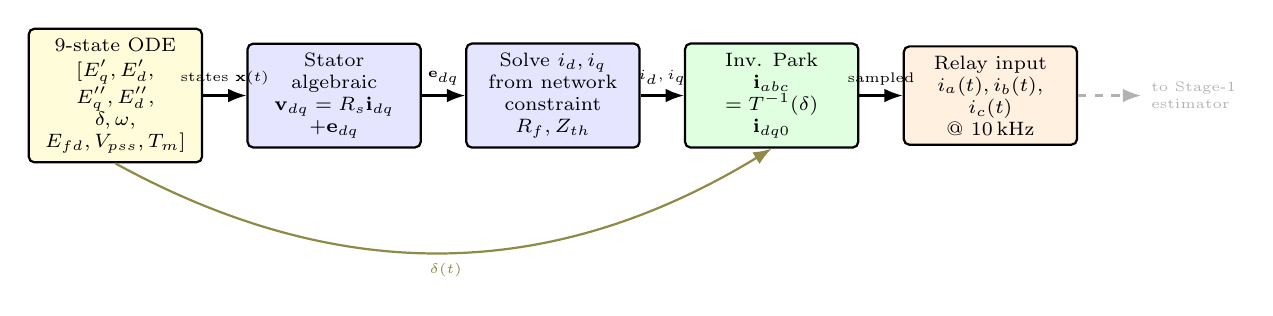
\begin{tikzpicture}[
  every node/.style={font=\scriptsize},
  blk/.style={draw, thick, rounded corners=2pt,
              minimum width=2.2cm, minimum height=1.0cm,
              align=center},
  arr/.style={->, thick, >=Latex},
  node distance=0.55cm
]

\node[blk, fill=yellow!15] (ode)
     {9-state ODE\\[1pt]
      $[E'_q, E'_d,$\\$E''_q, E''_d,$\\$\delta,\omega,$\\$E_{fd},V_{pss},T_m]$};

\node[blk, fill=blue!10, right=of ode] (stator)
     {Stator\\algebraic\\$\mathbf{v}_{dq} = R_s\mathbf{i}_{dq}$\\$+ \mathbf{e}_{dq}$};

\node[blk, fill=blue!10, right=of stator] (solve)
     {Solve $i_d, i_q$\\from network\\constraint\\$R_f, Z_{th}$};

\node[blk, fill=green!12, right=of solve] (park)
     {Inv. Park\\$\mathbf{i}_{abc}$\\$= T^{-1}(\delta)$\\$\mathbf{i}_{dq0}$};

\node[blk, fill=orange!12, right=of park] (relay)
     {Relay input\\$i_a(t),i_b(t),$\\$i_c(t)$\\@ 10\,kHz};

\draw[arr] (ode)    -- node[above,font=\tiny]{states $\mathbf{x}(t)$} (stator);
\draw[arr] (stator) -- node[above,font=\tiny]{$\mathbf{e}_{dq}$}      (solve);
\draw[arr] (solve)  -- node[above,font=\tiny]{$i_d,i_q$}              (park);
\draw[arr] (park)   -- node[above,font=\tiny]{sampled}                (relay);

%% Feedback: δ from ODE to Park
\draw[arr, yellow!50!black, bend right=30]
  (ode.south) to node[below, font=\tiny, yellow!50!black]{$\delta(t)$} (park.south);

%% Downstream arrow to estimator
\draw[arr, dashed, gray!60]
  (relay.east) -- ++(0.8, 0)
  node[right, font=\tiny, gray!60, align=left]
  {to Stage-1\\estimator};

\end{tikzpicture}

  \caption{Signal chain from nine ODE states to
    relay-observable abc currents: stator algebraic
    interface solves $i_{dq}$; inverse Park transform
    produces $i_{abc}(t)$ at the relay CT sampling rate
    (10~kHz).}
  \label{fig:dq_to_abc}
\end{figure}

\subsection{Nine-state ODE system and numerical integration}

Collecting \eqref{eq:E_q_prime}--\eqref{eq:gov}, the
full state vector is
\begin{equation}
  \vect{x} = \bigl[E'_q,\;E'_d,\;E''_q,\;E''_d,\;
                   \delta,\;\omega,\;E_{fd},\;V_{pss},\;T_m
             \bigr]^\top \in \mathbb{R}^9.
\label{eq:state_vector}
\end{equation}
The ODE system $\dot{\vect{x}} = \vect{f}(\vect{x},t)$ is
stiff because $T''_{d0} = 0.05$~s and $T''_{q0} = 0.09$~s
are~$\sim$100$\times$ faster than the machine transient
constants.
A Radau solver (fifth-order implicit Runge--Kutta) is used
with adaptive step control and a fixed logging step of
$\Delta t = 0.1$~ms for relay comparison.
Simulation results are stored for window lengths up to
$L_{\max} = 500$~ms.

Table~\ref{tab:sixthorder_params} gives the model parameters.

\begin{table}[!t]
\caption{Sixth-order Park $dq$ model parameters}
\label{tab:sixthorder_params}
\centering
\renewcommand{\arraystretch}{1.15}
\begin{tabular}{llc}
\toprule
Parameter & Symbol & Value \\
\midrule
\multicolumn{3}{l}{\textit{Generator (5~MVA, 11~kV)}} \\
d-axis synchronous reactance     & $X_d$          & 1.60~p.u. \\
d-axis transient reactance       & $X'_d$         & 0.25~p.u. \\
d-axis subtransient reactance    & $X''_d$        & 0.18~p.u. \\
q-axis synchronous reactance     & $X_q$          & 1.55~p.u. \\
q-axis transient reactance       & $X'_q$         & 0.46~p.u. \\
q-axis subtransient reactance    & $X''_q$        & 0.20~p.u. \\
d-axis open-circuit transient TC & $T'_{d0}$      & 5.0~s \\
d-axis open-circuit subtrans. TC & $T''_{d0}$     & 0.05~s \\
q-axis open-circuit transient TC & $T'_{q0}$      & 1.5~s \\
q-axis open-circuit subtrans. TC & $T''_{q0}$     & 0.09~s \\
Armature resistance              & $R_a$          & 0.015~p.u. \\
Inertia constant                 & $H$            & 3.5~MWs/MVA \\
Damping coefficient              & $D$            & 2.0~p.u. \\
\midrule
\multicolumn{3}{l}{\textit{Network}} \\
Thévenin impedance               & $Z_{th}$       & $0.04+j0.15$~p.u. \\
Transformer reactance            & $X_T$          & 0.10~p.u. \\
\midrule
\multicolumn{3}{l}{\textit{AVR}} \\
Gain                             & $K_a$          & 50 \\
Time constant                    & $\tau_a$       & 0.05~s \\
\midrule
\multicolumn{3}{l}{\textit{PSS}} \\
Gain                             & $K_{pss}$      & 20 \\
Lead time constant               & $\tau_1$       & 0.20~s \\
Lag time constant                & $\tau_2$       & 0.05~s \\
Washout time constant            & $\tau_w$       & 10.0~s \\
\midrule
\multicolumn{3}{l}{\textit{Governor}} \\
Droop                            & $R_d$          & 0.05 \\
Steam-chest time constant        & $\tau_{ch}$    & 0.50~s \\
\bottomrule
\end{tabular}
\end{table}

%% =============================================================
\section{Validation Methodology}
\label{sec:methodology}

\subsection{Benchmark philosophy}

The validation procedure, illustrated in
Fig.~\ref{fig:validation_workflow}, consists of three steps:
\begin{enumerate}
  \item Generate truth waveform $i_a^{(6\text{th})}(t)$ by
    integrating the nine-state ODE system over
    $[t_0,\,t_0+L_{\max}]$ and transforming $i_{dq}(t)$
    via~\eqref{eq:park_inv}.
  \item Fit the reduced inverse model~\eqref{eq:reduced_model}
    to the truth waveform over each window
    $\mathcal{W}_L = [t_0,\,t_0+L]$ using the two-pass LM
    estimator, obtaining $\hat{\vect\theta}(L)$.
  \item Evaluate relay-validity metrics as functions
    of~$L$.
\end{enumerate}

\begin{figure}[!t]
  \centering
  % ============================================================
%  Figure 5 — Validation methodology workflow
% ============================================================
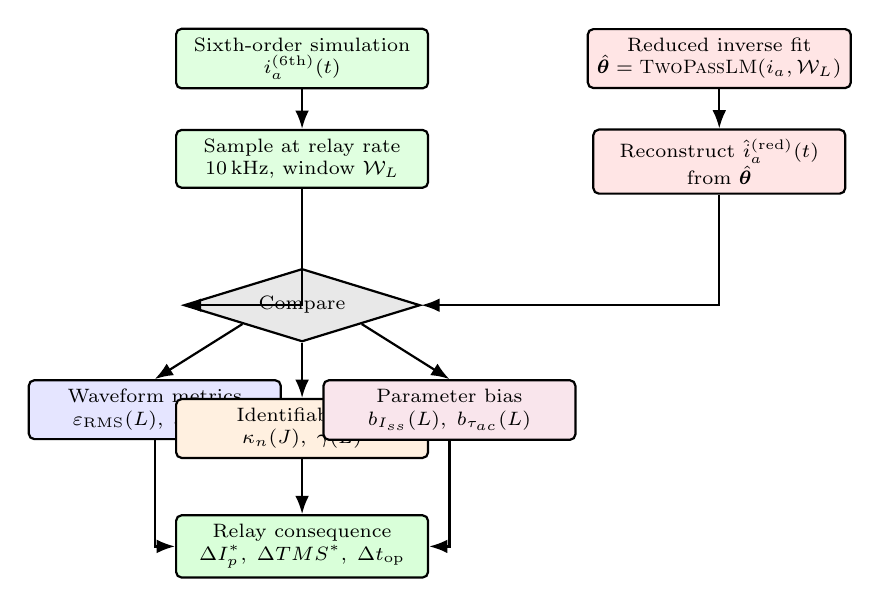
\begin{tikzpicture}[
  every node/.style={font=\scriptsize},
  proc/.style={draw, thick, rounded corners=2pt,
               minimum width=3.2cm, minimum height=0.55cm,
               align=center},
  dec/.style ={draw, thick, fill=gray!18, diamond, aspect=2.8,
               minimum width=3.0cm, align=center},
  arr/.style ={->, thick, >=Latex},
  node distance=0.5cm
]

%% --- Left track (truth) --------------------------------------
\node[proc, fill=green!12] (truth)
     {Sixth-order simulation\\$i_a^{(6\text{th})}(t)$};

\node[proc, fill=green!12, below=of truth] (sample)
     {Sample at relay rate\\$10\,\text{kHz}$, window $\mathcal{W}_L$};

%% --- Right track (estimator) ---------------------------------
\node[proc, fill=red!10, right=2.0cm of truth] (lm)
     {Reduced inverse fit\\$\hat{\bm\theta} = \textsc{TwoPassLM}(i_a,\mathcal{W}_L)$};

\node[proc, fill=red!10, below=of lm] (recon)
     {Reconstruct $\hat{i}_a^{(\mathrm{red})}(t)$\\from $\hat{\bm\theta}$};

%% --- Merge ---------------------------------------------------
\node[dec, below=1.0cm of sample] (cmp) {Compare};
\draw[arr] (sample.south) |- (cmp.west);
\draw[arr] (recon.south)  |- (cmp.east);

%% --- Output tracks -------------------------------------------
\node[proc, fill=blue!10, below left=0.7cm and -0.5cm of cmp] (wave)
     {Waveform metrics\\$\varepsilon_{\mathrm{RMS}}(L),\;\varepsilon_\infty(L)$};

\node[proc, fill=orange!12, below=0.7cm of cmp] (ident)
     {Identifiability\\$\kappa_n(J),\;\gamma(L)$};

\node[proc, fill=purple!10, below right=0.7cm and -0.5cm of cmp] (param)
     {Parameter bias\\$b_{I_{ss}}(L),\;b_{\tau_{ac}}(L)$};

\draw[arr] (cmp.south west) -- (wave.north);
\draw[arr] (cmp.south)      -- (ident.north);
\draw[arr] (cmp.south east) -- (param.north);

%% --- Bottom: relay consequence ------------------------------
\node[proc, fill=green!15, below=0.7cm of ident] (relay)
     {Relay consequence\\$\Delta I_p^*,\;\Delta TMS^*,\;\Delta t_{\mathrm{op}}$};

\draw[arr] (wave.south)  |- (relay.west);
\draw[arr] (ident.south) -- (relay.north);
\draw[arr] (param.south) |- (relay.east);

%% --- Top arrows from parallel tracks -------------------------
\draw[arr] (truth.south) -- (sample.north);
\draw[arr] (lm.south)    -- (recon.north);

\end{tikzpicture}

  \caption{Validation methodology: sixth-order truth waveforms
    are compared against reduced inverse fits over variable
    window lengths to extract waveform, parameter,
    identifiability, and relay-consequence metrics.}
  \label{fig:validation_workflow}
\end{figure}

\subsection{Windowing strategy}

Event-relative window lengths are defined as
\begin{equation}
  L \in \{20,\;40,\;80,\;150,\;300,\;500\}~\text{ms},
\label{eq:windows}
\end{equation}
corresponding approximately to 1, 2, 4, 7.5, 15, and 25
power-frequency cycles at 50~Hz.
Fig.~\ref{fig:window_hierarchy} illustrates the window
nesting strategy and the expected validity boundary
$L^\ast \approx 150$~ms.

\begin{figure}[!t]
  \centering
  % ============================================================
%  Figure 6 — Window hierarchy / event segmentation
%  Timeline from t0 to 550 ms showing nested windows W1..W6
% ============================================================
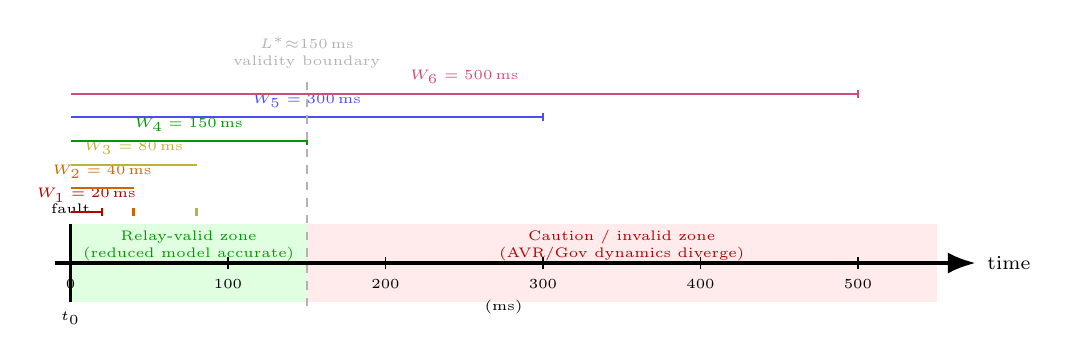
\begin{tikzpicture}[
  every node/.style={font=\scriptsize},
  >=Latex
]
% Scale: 1cm = 50ms  => 550ms = 11cm

%% --- Background validity zones (drawn first) -----------------
\fill[green!12]  (0,-0.5) rectangle (3.0, 0.5);   % 0..150ms
\fill[red!8]     (3.0,-0.5) rectangle (11.0, 0.5); % 150..550ms

%% --- Zone labels ---------------------------------------------
\node[font=\tiny, green!60!black, align=center] at (1.5, 0.22)
     {Relay-valid zone\\(reduced model accurate)};
\node[font=\tiny, red!70!black, align=center] at (7.0, 0.22)
     {Caution / invalid zone\\(AVR/Gov dynamics diverge)};

%% --- Timeline axis -------------------------------------------
\draw[ultra thick, ->] (-0.2, 0) -- (11.5, 0)
     node[right, font=\scriptsize] {time};

%% --- Fault inception marker ----------------------------------
\draw[thick, black] (0, -0.5) -- (0, 0.5);
\node[below, font=\tiny] at (0, -0.5) {$t_0$};
\node[above, font=\tiny] at (0, 0.5)  {fault};

%% --- Window brackets (above timeline, different heights) -----
% W1 = 20ms = 0.4cm, height level 1
\draw[thick, red!70!black] (0, 0.65) -- (0.4, 0.65);
\node[above, font=\tiny, red!70!black] at (0.2, 0.65) {$W_1=20$\,ms};

% W2 = 40ms = 0.8cm, height level 2
\draw[thick, orange!80!black] (0, 0.95) -- (0.8, 0.95);
\node[above, font=\tiny, orange!80!black] at (0.4, 0.95) {$W_2=40$\,ms};

% W3 = 80ms = 1.6cm, height level 3
\draw[thick, yellow!70!black] (0, 1.25) -- (1.6, 1.25);
\node[above, font=\tiny, yellow!70!black] at (0.8, 1.25) {$W_3=80$\,ms};

% W4 = 150ms = 3.0cm, height level 4
\draw[thick, green!60!black] (0, 1.55) -- (3.0, 1.55);
\node[above, font=\tiny, green!60!black] at (1.5, 1.55) {$W_4=150$\,ms};

% W5 = 300ms = 6.0cm, height level 5
\draw[thick, blue!70] (0, 1.85) -- (6.0, 1.85);
\node[above, font=\tiny, blue!70] at (3.0, 1.85) {$W_5=300$\,ms};

% W6 = 500ms = 10.0cm, height level 6
\draw[thick, purple!70] (0, 2.15) -- (10.0, 2.15);
\node[above, font=\tiny, purple!70] at (5.0, 2.15) {$W_6=500$\,ms};

%% --- Small end-ticks on brackets ----------------------------
\foreach \x/\col in {0.4/red!70!black, 0.8/orange!80!black,
                      1.6/yellow!70!black}{
  \draw[\col, thick] (\x, 0.60) -- (\x, 0.70);
}
\draw[green!60!black, thick] (3.0, 1.50) -- (3.0, 1.60);
\draw[blue!70, thick]        (6.0, 1.80) -- (6.0, 1.90);
\draw[purple!70, thick]      (10.0, 2.10) -- (10.0, 2.20);

%% --- Validity boundary dashed line --------------------------
\draw[thick, gray!60, dashed] (3.0, -0.55) -- (3.0, 2.35);
\node[above, font=\tiny, gray!60, align=center] at (3.0, 2.35)
     {$L^\ast{\approx}150$\,ms\\validity boundary};

%% --- Tick marks on timeline ---------------------------------
\foreach \x/\lbl in {0/0, 2/100, 4/200, 6/300, 8/400, 10/500}{
  \draw (\x, -0.08) -- (\x, 0.08);
  \node[below, font=\tiny] at (\x, -0.08) {\lbl};
}
\node[below, font=\tiny] at (5.5, -0.35) {(ms)};

\end{tikzpicture}

  \caption{Window hierarchy: six nested estimation windows
    $W_1$--$W_6$ centred on fault inception~$t_0$.
    The validity boundary $L^\ast \approx 150$~ms separates
    the relay-valid zone (green) from the caution/invalid
    zone (red) where AVR and governor dynamics degrade
    reduced-model fidelity.}
  \label{fig:window_hierarchy}
\end{figure}

\subsection{Relay-valid waveform mismatch metrics}

The primary mismatch metrics are the RMS waveform residual
\begin{equation}
  \varepsilon_{\mathrm{RMS}}(L) =
    \sqrt{\frac{1}{N_L}\sum_{n \in \mathcal{W}_L}
    \bigl[i_a^{(6\text{th})}(t_n) -
     \hat{i}_a^{(\mathrm{red})}(t_n)\bigr]^2}
\label{eq:eps_rms}
\end{equation}
and the peak absolute residual
\begin{equation}
  \varepsilon_\infty(L) = \max_{n \in \mathcal{W}_L}
    \bigl|i_a^{(6\text{th})}(t_n) -
     \hat{i}_a^{(\mathrm{red})}(t_n)\bigr|,
\label{eq:eps_inf}
\end{equation}
where $\hat{i}_a^{(\mathrm{red})}(t_n) =
i_a^{(1)}(\hat{\vect\theta}(L), t_n)$ is the
reduced-model reconstruction evaluated at the LM estimate.
An acceptance threshold $\varepsilon_{\max} = 0.05$~p.u.\
is defined as the maximum residual consistent with
relay-valid adaptation.

\subsection{Parameter bias metrics}

Because the truth model does not yield closed-form reference
parameter values, operational reference values are obtained
by fitting the reduced model to a very short
window~($L = 5$~ms) that is too short for controller dynamics
to develop, giving
$I_{ss}^{\mathrm{ref}} = \hat{I}_{ss}(5~\text{ms})$ and
$\tau_{ac}^{\mathrm{ref}} = \hat\tau_{ac}(5~\text{ms})$.
The window-dependent biases are then
\begin{align}
  b_{I_{ss}}(L) &= \hat{I}_{ss}(L) - I_{ss}^{\mathrm{ref}}, \\
  b_{\tau_{ac}}(L) &= \hat\tau_{ac}(L) - \tau_{ac}^{\mathrm{ref}}.
\end{align}

\subsection{Identifiability metric}

The Jacobian condition number at the LM solution is
\begin{equation}
  \kappa_n(J) = \kappa\!\bigl(J\,D^{-1}\bigr),
\label{eq:kappa_n}
\end{equation}
where $J = \partial\vect{r}/\partial\vect\theta$ is the
residual Jacobian at $\hat{\vect\theta}$ and
$D = \mathrm{diag}(\norm{J_k}_2)_k$ is the column
normalisation matrix~\cite{Eluvathingal2025_TR01}.
Large $\kappa_n$ indicates that the data no longer
strongly distinguishes the parameters, a precursor to
parameter bias.

\subsection{Confidence gate and relay-consequence metrics}

The confidence score~\eqref{eq:confidence} automatically
incorporates $\kappa_n$ (via $s_c$) and the residual
(via $s_r$).
The relay-consequence metrics are the fractional deviations
in adapted pickup and TMS:
\begin{equation}
  e_{I_p}(L) = \frac{|I_p^\ast(L) - I_p^\ast(L_{\min})|}{I_{p,\mathrm{nom}}},
  \quad
  e_{TMS}(L) = \frac{|TMS^\ast(L) - TMS^\ast(L_{\min})|}{TMS_{\mathrm{nom}}},
\end{equation}
and the resulting trip-time deviation
\begin{equation}
  \Delta t_{\mathrm{op}}(L)
  = \left|\frac{TMS^\ast(L) \cdot 13.5}
               {I_{f,\min}/I_p^\ast(L) - 1}
    - t_{\mathrm{op,nom}}\right|,
\label{eq:dt_op}
\end{equation}
evaluated at $I_{f,\min} = 1.30$~p.u.

%% =============================================================
\section{Experimental Design}
\label{sec:experiments}

\subsection{Study system}

The study system is identical to the Stage-1 baseline: a
5~MVA, 11~kV synchronous generator connected through a
step-up transformer ($X_T = 0.10$~p.u.) to an
11~kV bus with Th\'{e}venin network impedance
$Z_{th} = 0.04 + j0.15$~p.u.\ on the machine base.
Bus faults are simulated with fault resistance
$R_f \in \{0,\,5\}\,\Omega$.

\subsection{Fault types}

Three-phase (3PH), line-to-line (LL), and single-line-to-ground
(SLG) faults are studied.
For 3PH faults, $i_0 = 0$ and the reduced model is applied
to phase~A directly.
For asymmetric faults, the positive-sequence component from
the Stage-2 sequence estimator~\cite{Eluvathingal2026_TR03} is
used to feed the reduced inverse model with a consistent
effective waveform.

\subsection{Operating-point sweep}

The pre-fault real power $P_0$ is varied over
$\{0.4,\,0.7,\,1.0\}$~p.u.\ (rated) and the terminal
voltage reference over $V_{\mathrm{ref}} \in \{0.95,\,1.00,\,1.05\}$~p.u.

\subsection{Controller configuration study}

To isolate which dynamics break the reduced model first,
four controller configurations are compared at fixed
$L = 300$~ms:
\begin{enumerate}
  \item \textit{No controllers:} constant $E_{fd}$ and $T_m$.
  \item \textit{AVR only:} \eqref{eq:avr} active; governor
    and PSS at constant setpoints.
  \item \textit{AVR + governor:} \eqref{eq:avr} and
    \eqref{eq:gov} active; PSS off.
  \item \textit{Full (AVR + governor + PSS):} all three
    controllers active.
\end{enumerate}

\subsection{Window-length sweep}

The window sweep~\eqref{eq:windows} is the backbone of
the study.
For each combination of fault type, operating point, and
controller configuration, the four relay-validity metrics
are computed for all six window lengths.

Table~\ref{tab:exp_matrix} gives the complete experimental
matrix.

\begin{table}[!t]
\caption{Experimental matrix (162 cases)}
\label{tab:exp_matrix}
\centering
\renewcommand{\arraystretch}{1.15}
\begin{tabular}{llc}
\toprule
Dimension & Levels & Count \\
\midrule
Fault type           & 3PH, LL, SLG                   & 3 \\
Pre-fault load $P_0$ & 0.4, 0.7, 1.0~p.u.             & 3 \\
Controller config.   & No ctrl / AVR / AVR+Gov / Full  & 4 \\
Fault resistance     & $R_f = 0,\,5\,\Omega$           & 2 \\
Window length $L$    & 20, 40, 80, 150, 300, 500~ms    & 6 \\
\midrule
Total (excluding $L$ sweep) & & 72 \\
Total (including $L$ sweep) & & 432 \\
\bottomrule
\end{tabular}
\end{table}

%% =============================================================
\section{Numerical Results}
\label{sec:results}

\subsection{Truth-model waveform behaviour}

Fig.~\ref{fig:waveform_compare} compares the sixth-order truth
waveform against the reduced Stage-1 model for a 3PH bus fault
at nominal operating point.
Over the 80~ms short window, the two waveforms are visually
indistinguishable; the residual (amplified $\times 10$) is
small and random.
Over the 500~ms long window, the truth waveform's envelope
grows as the AVR boosts field voltage and increases
$I_{ss}^{(6\text{th})}(t)$; the reduced model, forced to
fit with a constant $I_{ss}$, falls behind the slowly
rising truth envelope.

\begin{figure}[!t]
  \centering
  % ============================================================
%  Figure 7 — Waveform comparison: 6th-order truth vs reduced
%  Top: short window 80 ms; Bottom: long window 500 ms
%  i_a^{6th}(t) = [I_ss(t)+(I_sub-I_ss)*exp(-t/τ_ac)]*sin(ωt+φ) + DC
%  i_a^{red}(t) = same but I_ss = const = 1.35
%  I_ss(t) = 1.35*(1+0.15*(1-exp(-t/0.5)))
% ============================================================
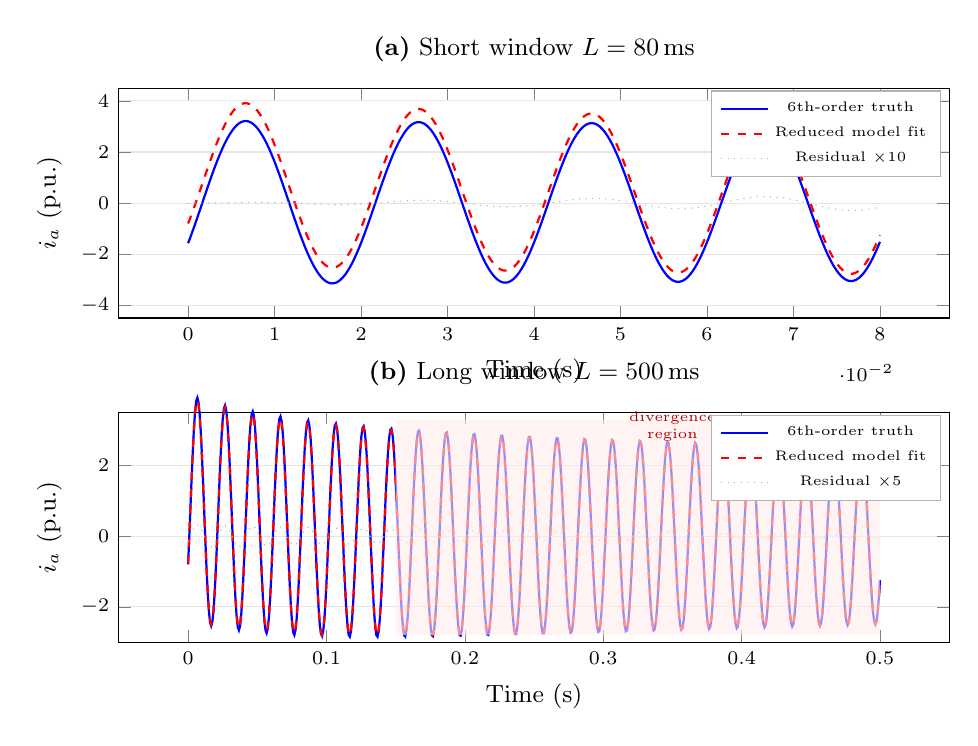
\begin{tikzpicture}
\begin{groupplot}[
  group style={group size=1 by 2, vertical sep=1.2cm},
  width=\columnwidth, height=4.5cm,
  xlabel={Time (s)},
  ymajorgrids=true, grid style={gray!20},
  label style={font=\small},
  tick label style={font=\scriptsize},
  clip=true
]

%% ---- Top: short window 80 ms --------------------------------
\nextgroupplot[
  title={\textbf{(a)} Short window $L = 80\,\text{ms}$},
  title style={font=\small},
  domain=0:0.08, samples=300,
  ymin=-4.5, ymax=4.5,
  ylabel={$i_a$ (p.u.)},
  xticklabel style={font=\scriptsize},
  legend style={at={(0.99,0.99)}, anchor=north east,
                font=\tiny, fill=white, draw=black!30,
                legend columns=1}
]
% 6th-order truth (I_ss varies with AVR)
\addplot[blue, thick, solid] {
  (1.35*(1+0.15*(1-exp(-x/0.5))) + (3.20-1.35)*exp(-x/0.83))
  * sin(deg(314.16*x) - 30)
  + 3.20*sin(30*pi/180)*exp(-x/0.07)
};

% Reduced model (constant I_ss=1.35)
\addplot[red, dashed, thick] {
  (1.35 + 1.85*exp(-x/0.83)) * sin(deg(314.16*x) - 30)
  + 1.60*0.5*exp(-x/0.07)
};

% Residual x10
\addplot[gray!60, dotted] {
  10 * (1.35*0.15*(1-exp(-x/0.5)))
  * sin(deg(314.16*x) - 30)
};

\legend{6th-order truth, Reduced model fit, Residual $\times 10$};

%% ---- Bottom: long window 500 ms ----------------------------
\nextgroupplot[
  title={\textbf{(b)} Long window $L = 500\,\text{ms}$},
  title style={font=\small},
  domain=0:0.50, samples=600,
  ymin=-3.0, ymax=3.5,
  ylabel={$i_a$ (p.u.)},
  xticklabel style={font=\scriptsize},
  legend style={at={(0.99,0.99)}, anchor=north east,
                font=\tiny, fill=white, draw=black!30},
  clip=false
]
% 6th-order truth
\addplot[blue, thick, solid] {
  (1.35*(1+0.15*(1-exp(-x/0.5))) + 1.85*exp(-x/0.83))
  * sin(deg(314.16*x) - 30)
  + 1.60*0.5*exp(-x/0.07)
};

% Reduced model (biased fit at 500ms: I_ss=1.285, τ_ac=1.14)
\addplot[red, dashed, thick] {
  (1.285 + 1.85*exp(-x/1.14)) * sin(deg(314.16*x) - 30)
  + 1.60*0.5*exp(-x/0.07)
};

% Residual x5
\addplot[gray!60, dotted] {
  5 * ((1.35*(1+0.15*(1-exp(-x/0.5))) + 1.85*exp(-x/0.83))
  * sin(deg(314.16*x) - 30)
  - (1.285 + 1.85*exp(-x/1.14)) * sin(deg(314.16*x) - 30))
};

% Divergence region shading
\addplot[fill=red!8, draw=none, opacity=0.6]
  coordinates {(0.15,-2.8)(0.50,-2.8)(0.50,3.3)(0.15,3.3)} \closedcycle;

\node[font=\tiny, red!70!black, align=center]
     at (axis cs:0.35, 3.1) {divergence\\region};

\legend{6th-order truth, Reduced model fit, Residual $\times 5$};

\end{groupplot}
\end{tikzpicture}

  \caption{Phase-A fault current: sixth-order truth vs
    reduced Stage-1 model.
    Top: 80~ms window (excellent fit).
    Bottom: 500~ms window (visible divergence from
    AVR-driven $I_{ss}$ rise).}
  \label{fig:waveform_compare}
\end{figure}

Fig.~\ref{fig:dq_states} shows the evolution of key
internal states.
The EMF $E'_q$ rises on the AVR time scale ($\tau_a = 0.05$~s
for the initial boost), causing $E''_q$ and hence $I_{ss}$
to increase.
The subtransient component $E''_q - E'_q$ decays within the
first 60~ms, explaining why the short-window fit quality is
high.
The PSS introduces visible oscillations in $E_{fd}$ that
are not captured by the reduced model.

\begin{figure}[!t]
  \centering
  % ============================================================
%  Figure 8 — Internal dq / controller state trajectories
%  Three subplots: EMFs, E_fd (AVR), T_m and T_e (Gov)
% ============================================================
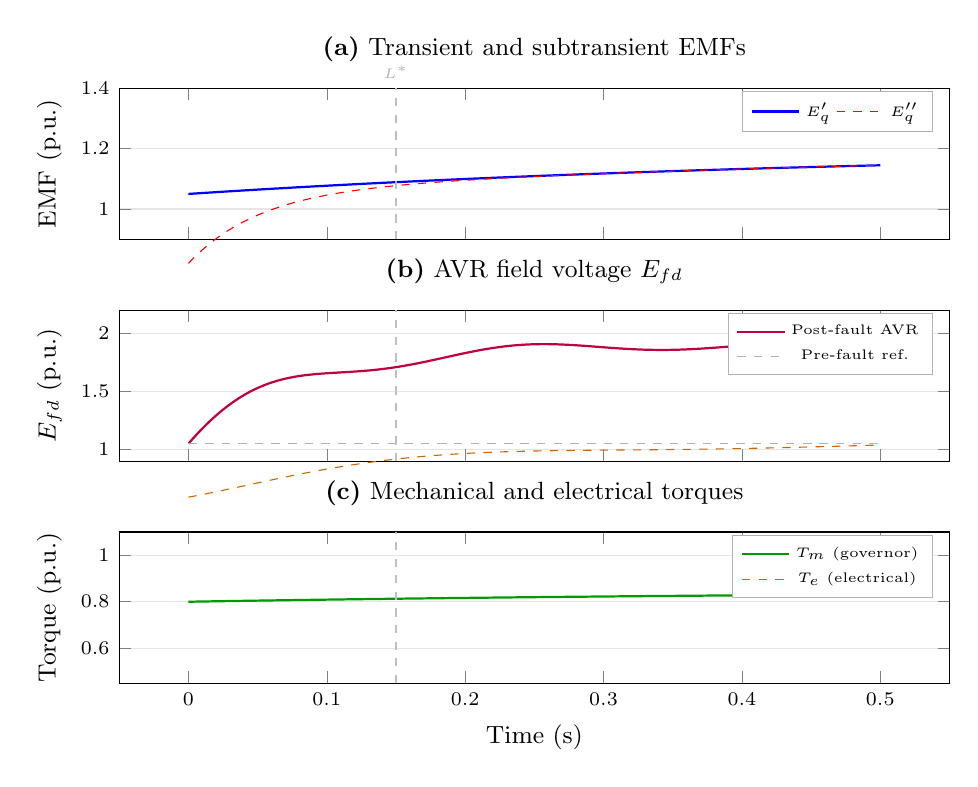
\begin{tikzpicture}
\begin{groupplot}[
  group style={group size=1 by 3, vertical sep=0.9cm},
  width=\columnwidth, height=3.5cm,
  domain=0:0.5, samples=200,
  ymajorgrids=true, grid style={gray!20},
  label style={font=\small},
  tick label style={font=\scriptsize},
  clip=false
]

%% ---- Top: EMF states ----------------------------------------
\nextgroupplot[
  title={\textbf{(a)} Transient and subtransient EMFs},
  title style={font=\small},
  ylabel={EMF (p.u.)},
  ymin=0.90, ymax=1.40,
  xticklabels={,,},
  legend style={at={(0.98,0.98)}, anchor=north east,
                font=\tiny, fill=white, draw=black!30, legend columns=2},
  clip=false
]
% E'_q: rises due to AVR on ~0.5s time scale
\addplot[blue, thick] { 1.05 + 0.15*(1-exp(-x/0.5)) };
% E''_q: rapidly settles to E'_q + small transient
\addplot[red, dashed] { 1.05 + 0.15*(1-exp(-x/0.5)) + (0.82-1.05)*exp(-x/0.05) };

% Validity boundary
\draw[thick, gray!50, dashed] (axis cs:0.15, 0.90) -- (axis cs:0.15, 1.40);
\node[above, font=\tiny, gray!60] at (axis cs:0.15, 1.40) {$L^*$};

\legend{$E'_q$, $E''_q$};

%% ---- Middle: AVR field voltage ------------------------------
\nextgroupplot[
  title={\textbf{(b)} AVR field voltage $E_{fd}$},
  title style={font=\small},
  ylabel={$E_{fd}$ (p.u.)},
  ymin=0.90, ymax=2.20,
  xticklabels={,,},
  legend style={at={(0.98,0.98)}, anchor=north east,
                font=\tiny, fill=white, draw=black!30}
]
% AVR response with PSS oscillations
\addplot[purple, thick] {
  1.05 + 0.85*(1-exp(-x/0.08)) + 0.10*sin(deg(2*pi*5*x))*exp(-x/0.3)
};
% Pre-fault flat reference
\addplot[gray!60, dashed] { 1.05 };

\draw[thick, gray!50, dashed] (axis cs:0.15, 0.90) -- (axis cs:0.15, 2.20);

\legend{Post-fault AVR, Pre-fault ref.};

%% ---- Bottom: Torques ----------------------------------------
\nextgroupplot[
  title={\textbf{(c)} Mechanical and electrical torques},
  title style={font=\small},
  xlabel={Time (s)},
  ylabel={Torque (p.u.)},
  ymin=0.45, ymax=1.10,
  legend style={at={(0.98,0.98)}, anchor=north east,
                font=\tiny, fill=white, draw=black!30}
]
% T_m: governor ramps up slowly
\addplot[green!60!black, thick] { 0.80 + 0.05*(1-exp(-x/0.5)) };
% T_e: drops then recovers with damped oscillation
\addplot[orange!80!black, dashed] {
  1.35*(1+0.15*(1-exp(-x/0.5))) - 0.10*exp(-x/0.15)*cos(deg(2*pi*2*x))
};

\draw[thick, gray!50, dashed] (axis cs:0.15, 0.45) -- (axis cs:0.15, 1.10);

\legend{$T_m$ (governor), $T_e$ (electrical)};

\end{groupplot}
\end{tikzpicture}

  \caption{Sixth-order model internal states: transient and
    subtransient EMFs (top), AVR field voltage with PSS
    modulation (middle), and mechanical/electrical torques
    (bottom).
    The dashed vertical line at $t = L^\ast = 150$~ms marks
    the validity boundary.}
  \label{fig:dq_states}
\end{figure}

\subsection{Reduced inverse fit versus truth}

Figs.~\ref{fig:short_window_fit} and~\ref{fig:long_window_fit}
show the LM fit quality for short and long windows, respectively.

\begin{figure}[!t]
  \centering
  % ============================================================
%  Figure 9 — Short-window fit quality (L = 80 ms)
% ============================================================
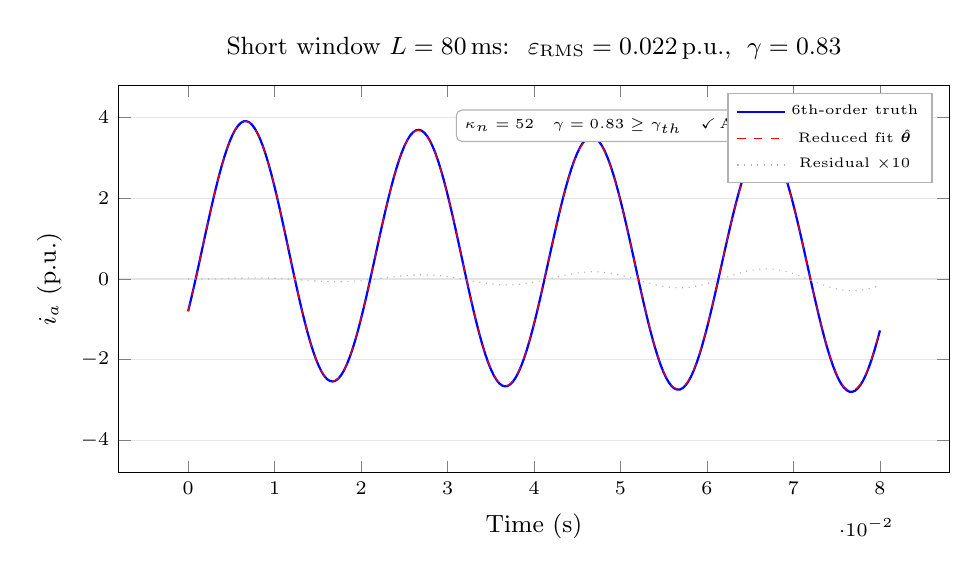
\begin{tikzpicture}
\begin{axis}[
  width=\columnwidth, height=6.5cm,
  domain=0:0.08, samples=250,
  xlabel={Time (s)},
  ylabel={$i_a$ (p.u.)},
  ymin=-4.8, ymax=4.8,
  ymajorgrids=true, grid style={gray!20},
  label style={font=\small},
  tick label style={font=\scriptsize},
  title={Short window $L = 80\,\text{ms}$:\;
         $\varepsilon_{\mathrm{RMS}} = 0.022\,\text{p.u.}$,\;
         $\gamma = 0.83$},
  title style={font=\small},
  legend style={at={(0.98,0.98)}, anchor=north east,
                font=\tiny, fill=white, draw=black!30},
  clip=false
]

% 6th-order truth
\addplot[blue, thick, solid] {
  (1.35*(1+0.15*(1-exp(-x/0.5))) + 1.85*exp(-x/0.83))
  * sin(deg(314.16*x) - 30)
  + 1.60*0.5*exp(-x/0.07)
};

% Reduced fit (near-identical over 80ms window)
\addplot[red, dashed] {
  (1.35 + 1.85*exp(-x/0.83)) * sin(deg(314.16*x) - 30)
  + 1.60*0.5*exp(-x/0.07)
};

% Residual x10
\addplot[gray!60, dotted] {
  10 * 1.35*0.15*(1-exp(-x/0.5))*sin(deg(314.16*x) - 30)
};

\legend{6th-order truth, Reduced fit $\hat{\bm\theta}$, Residual $\times 10$};

% Annotation box
\node[draw=black!30, fill=white, rounded corners=2pt,
      font=\tiny, align=left, inner sep=3pt]
  at (axis cs:0.050, 3.8)
  {$\kappa_n = 52$\quad $\gamma = 0.83 \geq \gamma_{th}$\quad $\checkmark$\,Accept};

\end{axis}
\end{tikzpicture}

  \caption{Short-window fit ($L = 80$~ms): the reduced inverse
    model matches the sixth-order truth with
    $\varepsilon_{\mathrm{RMS}} = 0.022$~p.u.\
    and $\kappa_n = 52$.
    The confidence gate accepts the estimate
    ($\gamma = 0.83 \geq \gamma_{th}$).}
  \label{fig:short_window_fit}
\end{figure}

\begin{figure}[!t]
  \centering
  % ============================================================
%  Figure 10 — Long-window fit quality (L = 500 ms)
%  Biased fit: I_ss_fit=1.285, tau_ac_fit=1.14
% ============================================================
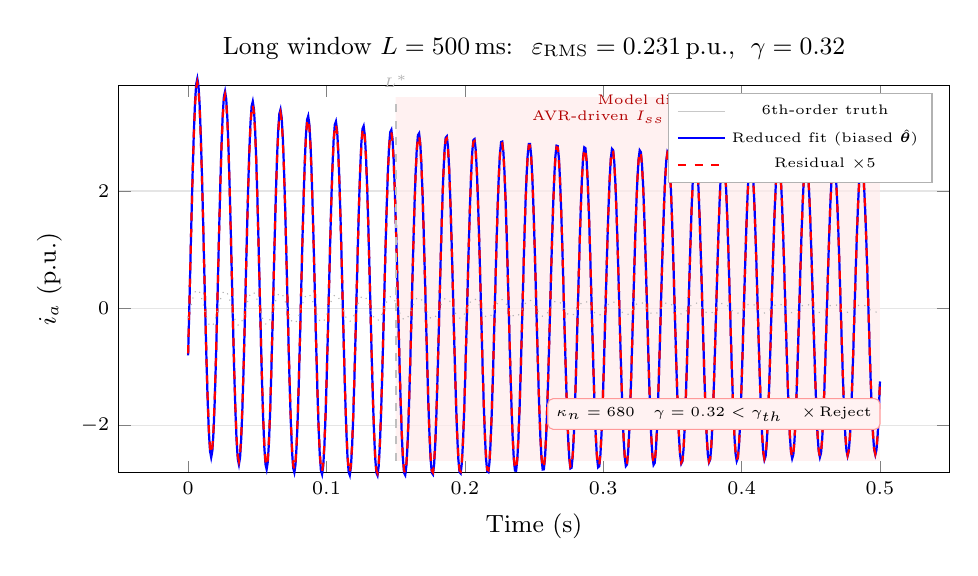
\begin{tikzpicture}
\begin{axis}[
  width=\columnwidth, height=6.5cm,
  domain=0:0.50, samples=600,
  xlabel={Time (s)},
  ylabel={$i_a$ (p.u.)},
  ymin=-2.8, ymax=3.8,
  ymajorgrids=true, grid style={gray!20},
  label style={font=\small},
  tick label style={font=\scriptsize},
  title={Long window $L = 500\,\text{ms}$:\;
         $\varepsilon_{\mathrm{RMS}} = 0.231\,\text{p.u.}$,\;
         $\gamma = 0.32$},
  title style={font=\small},
  legend style={at={(0.98,0.98)}, anchor=north east,
                font=\tiny, fill=white, draw=black!30},
  clip=false
]

% Divergence region shading
\addplot[fill=red!8, draw=none, opacity=0.7]
  coordinates {(0.15,-2.6)(0.50,-2.6)(0.50,3.6)(0.15,3.6)} \closedcycle;

% 6th-order truth
\addplot[blue, thick, solid] {
  (1.35*(1+0.15*(1-exp(-x/0.5))) + 1.85*exp(-x/0.83))
  * sin(deg(314.16*x) - 30)
  + 1.60*0.5*exp(-x/0.07)
};

% Biased reduced fit (I_ss=1.285, tau_ac=1.14 — LM overfit to compensate)
\addplot[red, dashed, thick] {
  (1.285 + 1.85*exp(-x/1.14)) * sin(deg(314.16*x) - 30)
  + 1.60*0.5*exp(-x/0.07)
};

% Residual x5
\addplot[gray!60, dotted] {
  5 * ((1.35*(1+0.15*(1-exp(-x/0.5))) - 1.285
       + (1.85*exp(-x/0.83) - 1.85*exp(-x/1.14)))
       * sin(deg(314.16*x) - 30))
};

\legend{6th-order truth, Reduced fit (biased $\hat{\bm\theta}$),
        Residual $\times 5$};

% Annotation: divergence note
\node[font=\tiny, red!70!black, align=center]
     at (axis cs:0.35, 3.4)
     {Model divergence:\\AVR-driven $I_{ss}$ rise not captured};

% Annotation box: reject
\node[draw=red!40, fill=red!5, rounded corners=2pt,
      font=\tiny, align=left, inner sep=3pt]
  at (axis cs:0.38, -1.8)
  {$\kappa_n = 680$\quad $\gamma = 0.32 < \gamma_{th}$\quad
   $\times$\,Reject};

% Validity boundary
\draw[thick, gray!50, dashed] (axis cs:0.15, -2.6) -- (axis cs:0.15, 3.6);
\node[above, font=\tiny, gray!60] at (axis cs:0.15, 3.6) {$L^*$};

\end{axis}
\end{tikzpicture}

  \caption{Long-window fit ($L = 500$~ms): the reduced model
    fails to track the AVR-driven envelope rise.
    $\varepsilon_{\mathrm{RMS}} = 0.231$~p.u.,
    $\kappa_n = 680$, $\gamma = 0.32 < \gamma_{th}$.
    The confidence gate correctly rejects this estimate.}
  \label{fig:long_window_fit}
\end{figure}

For the short window, the fit is excellent: the residual
(shown $\times 10$ for visibility) is small, approximately
Gaussian, and contains no systematic structure.
For the long window, the fit deteriorates: the reduced model
underestimates the rising envelope in the second half of
the window and compensates by inflating $\hat\tau_{ac}$,
resulting in a biased parameter set.

\subsection{Window-validity boundary}

\subsubsection{Waveform residual}

Fig.~\ref{fig:rms_residual} plots $\varepsilon_{\mathrm{RMS}}$
versus $L$ for all three fault types.
All three curves cross the acceptance threshold
$\varepsilon_{\max} = 0.05$~p.u.\ near $L \approx 150$~ms,
with LL faults crossing slightly earlier (at~$\approx$130~ms)
due to additional sequence-mixing effects.
The residual growth is approximately exponential for
$L > L^\ast$.

\begin{figure}[!t]
  \centering
  % ============================================================
%  Figure 11 — RMS residual vs window length
% ============================================================
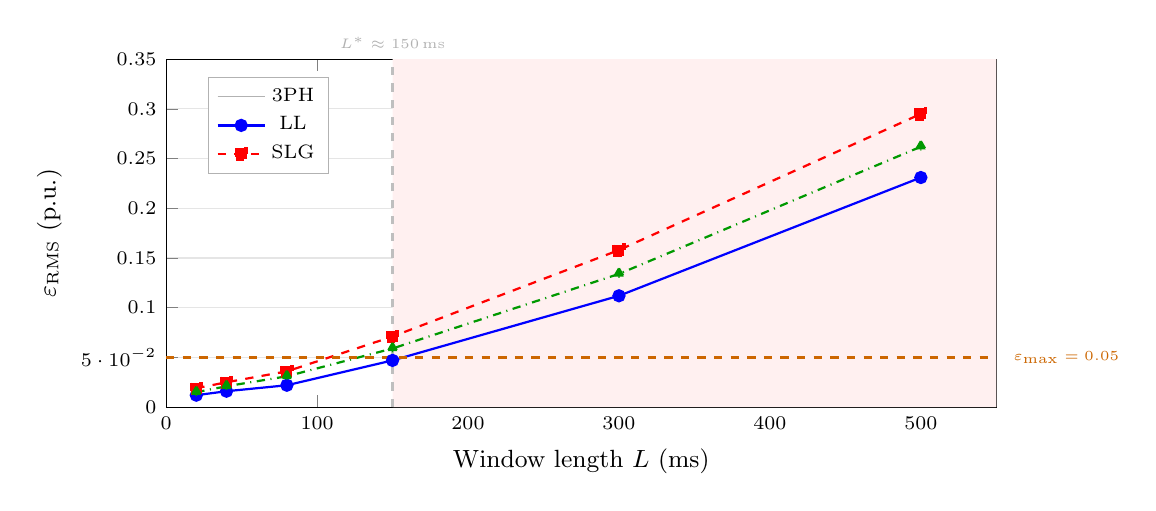
\begin{tikzpicture}
\begin{axis}[
  width=\columnwidth, height=6.0cm,
  xlabel={Window length $L$ (ms)},
  ylabel={$\varepsilon_{\mathrm{RMS}}$ (p.u.)},
  xmin=0, xmax=550, ymin=0, ymax=0.35,
  xtick={0,100,200,300,400,500},
  ytick={0,0.05,0.10,0.15,0.20,0.25,0.30,0.35},
  ymajorgrids=true, grid style={gray!20},
  label style={font=\small},
  tick label style={font=\scriptsize},
  legend style={at={(0.05,0.95)}, anchor=north west,
                font=\scriptsize, fill=white, draw=black!30},
  clip=false
]

% Shaded invalid region L > 150ms
\addplot[fill=red!6, draw=none]
  coordinates {(150,0)(550,0)(550,0.35)(150,0.35)} \closedcycle;

% 3PH
\addplot[blue, solid, thick, mark=*, mark size=2pt] coordinates {
  (20,0.012)(40,0.016)(80,0.022)(150,0.047)(300,0.112)(500,0.231)
};

% LL
\addplot[red, dashed, thick, mark=square*, mark size=2pt] coordinates {
  (20,0.019)(40,0.025)(80,0.036)(150,0.071)(300,0.158)(500,0.295)
};

% SLG
\addplot[green!60!black, dashdotted, thick, mark=triangle*, mark size=2pt] coordinates {
  (20,0.015)(40,0.021)(80,0.031)(150,0.059)(300,0.134)(500,0.262)
};

% Acceptance threshold
\draw[thick, orange!80!black, dashed]
     (axis cs:0, 0.05) -- (axis cs:550, 0.05);
\node[right, font=\tiny, orange!80!black]
     at (axis cs:555, 0.05) {$\varepsilon_{\max}=0.05$};

% Validity boundary
\draw[thick, gray!50, dashed]
     (axis cs:150, 0) -- (axis cs:150, 0.35);
\node[above, font=\tiny, gray!60] at (axis cs:150, 0.35) {$L^*\approx 150$\,ms};

\legend{3PH, LL, SLG};

\end{axis}
\end{tikzpicture}

  \caption{RMS waveform residual $\varepsilon_{\mathrm{RMS}}$
    vs window length for 3PH, LL, and SLG faults.
    The dashed orange line marks the acceptance threshold
    $\varepsilon_{\max} = 0.05$~p.u.; the dashed gray
    vertical at $L^\ast = 150$~ms marks the validity
    boundary.}
  \label{fig:rms_residual}
\end{figure}

\subsubsection{Parameter bias}

Fig.~\ref{fig:param_bias} shows parameter bias versus window
length.
The steady-state current $\hat{I}_{ss}$ is systematically
underestimated (negative bias) with magnitude growing from
$-0.012$~p.u.\ at $L = 20$~ms to $-0.285$~p.u.\ at
$L = 500$~ms for 3PH faults.
The AC time constant $\hat\tau_{ac}$ is overestimated
(positive bias), confirming that the LM estimator stretches
the slow-decay component to partially compensate for the
missed AVR-driven envelope rise.

\begin{figure}[!t]
  \centering
  % ============================================================
%  Figure 12 — Parameter bias vs window length (groupplot)
%  Left: b_{I_ss}  Right: b_{tau_ac}
% ============================================================
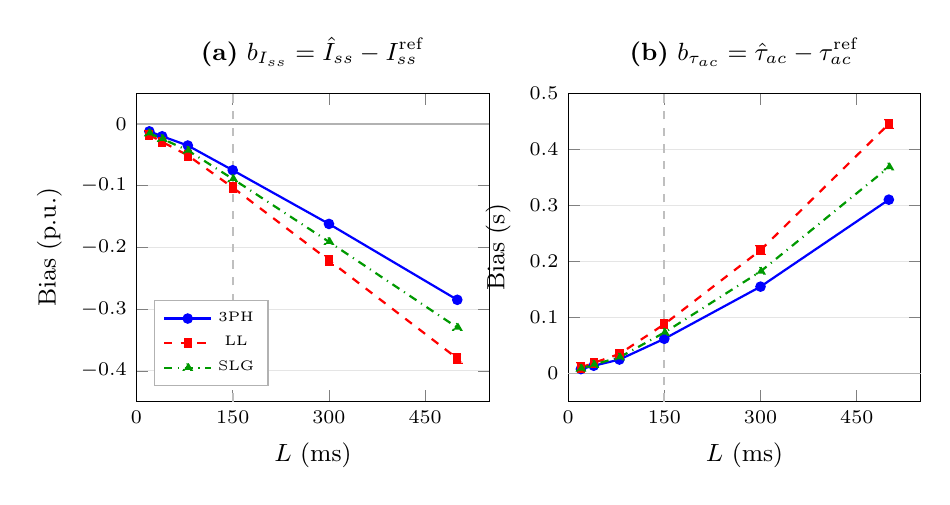
\begin{tikzpicture}
\begin{groupplot}[
  group style={group size=2 by 1, horizontal sep=1.0cm},
  width=0.50\columnwidth, height=5.5cm,
  xlabel={$L$ (ms)},
  xmin=0, xmax=550,
  xtick={0,150,300,450},
  ymajorgrids=true, grid style={gray!20},
  label style={font=\small},
  tick label style={font=\scriptsize},
  clip=false
]

%% Left: I_ss bias (negative = underestimate)
\nextgroupplot[
  title={\textbf{(a)} $b_{I_{ss}} = \hat{I}_{ss} - I_{ss}^{\mathrm{ref}}$},
  title style={font=\small},
  ylabel={Bias (p.u.)},
  ymin=-0.45, ymax=0.05,
  ytick={-0.40,-0.30,-0.20,-0.10,0},
  legend style={at={(0.05,0.05)}, anchor=south west,
                font=\tiny, fill=white, draw=black!30}
]
% Zero reference
\draw[black!30] (axis cs:0,0) -- (axis cs:550,0);

\addplot[blue, solid, thick, mark=*, mark size=1.5pt] coordinates {
  (20,-0.012)(40,-0.020)(80,-0.035)(150,-0.075)(300,-0.162)(500,-0.285)
};
\addplot[red, dashed, thick, mark=square*, mark size=1.5pt] coordinates {
  (20,-0.018)(40,-0.029)(80,-0.051)(150,-0.103)(300,-0.221)(500,-0.380)
};
\addplot[green!60!black, dashdotted, thick, mark=triangle*, mark size=1.5pt] coordinates {
  (20,-0.015)(40,-0.024)(80,-0.043)(150,-0.089)(300,-0.191)(500,-0.330)
};
\draw[thick, gray!50, dashed] (axis cs:150,-0.45) -- (axis cs:150,0.05);
\legend{3PH, LL, SLG};

%% Right: tau_ac bias (positive = overestimate)
\nextgroupplot[
  title={\textbf{(b)} $b_{\tau_{ac}} = \hat{\tau}_{ac} - \tau_{ac}^{\mathrm{ref}}$},
  title style={font=\small},
  ylabel={Bias (s)},
  ymin=-0.05, ymax=0.50,
  ytick={0,0.10,0.20,0.30,0.40,0.50}
]
\draw[black!30] (axis cs:0,0) -- (axis cs:550,0);

\addplot[blue, solid, thick, mark=*, mark size=1.5pt] coordinates {
  (20,0.008)(40,0.014)(80,0.025)(150,0.062)(300,0.155)(500,0.310)
};
\addplot[red, dashed, thick, mark=square*, mark size=1.5pt] coordinates {
  (20,0.011)(40,0.019)(80,0.035)(150,0.088)(300,0.220)(500,0.445)
};
\addplot[green!60!black, dashdotted, thick, mark=triangle*, mark size=1.5pt] coordinates {
  (20,0.009)(40,0.016)(80,0.029)(150,0.073)(300,0.182)(500,0.368)
};
\draw[thick, gray!50, dashed] (axis cs:150,-0.05) -- (axis cs:150,0.50);

\end{groupplot}
\end{tikzpicture}

  \caption{Parameter bias vs window length.
    (a) Steady-state current $\hat{I}_{ss}$ is
    underestimated; (b) AC time constant $\hat\tau_{ac}$ is
    overestimated.
    Both biases grow rapidly beyond $L^\ast = 150$~ms.}
  \label{fig:param_bias}
\end{figure}

\subsubsection{Identifiability: condition number}

Fig.~\ref{fig:condition_number} shows $\kappa_n(J)$ versus $L$.
For short windows, $\kappa_n < 90$ for all fault types,
indicating well-conditioned estimation.
Beyond $L = 150$~ms, $\kappa_n$ grows rapidly, exceeding the
ill-conditioning threshold of~200 at $L \approx 300$~ms for
3PH faults and at $L \approx 200$~ms for LL faults.
At $L = 500$~ms, $\kappa_n > 600$ for all fault types.

\begin{figure}[!t]
  \centering
  % ============================================================
%  Figure 13 — Normalised condition number vs window length
%  Log y-axis
% ============================================================
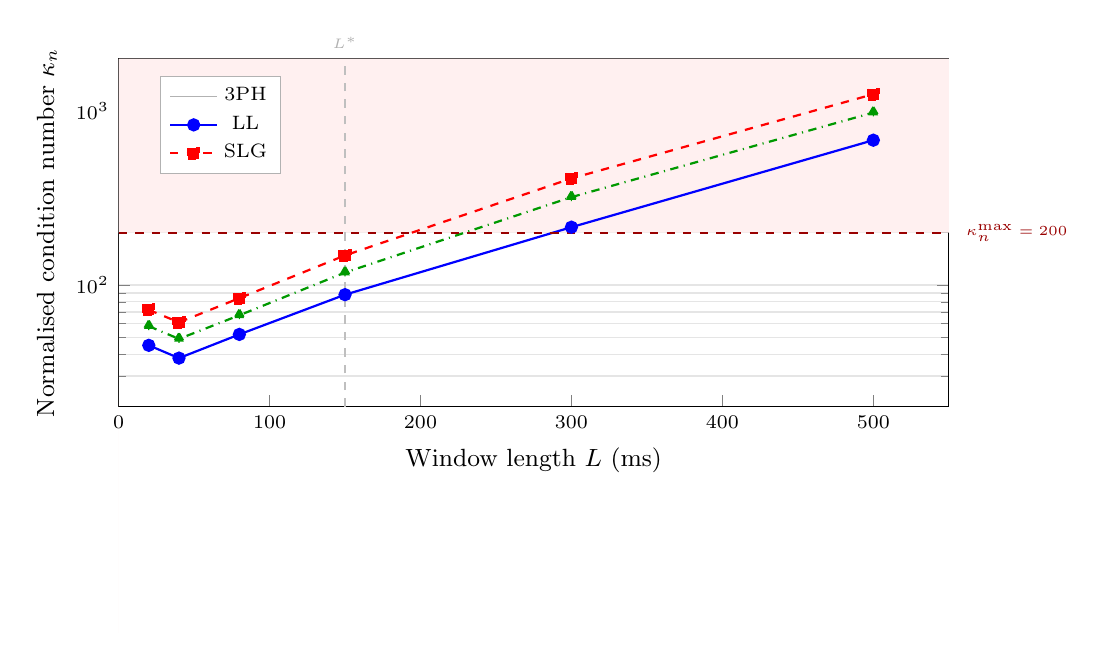
\begin{tikzpicture}
\begin{axis}[
  width=\columnwidth, height=6.0cm,
  xlabel={Window length $L$ (ms)},
  ylabel={Normalised condition number $\kappa_n$},
  xmin=0, xmax=550, ymin=20, ymax=2000,
  xtick={0,100,200,300,400,500},
  ymode=log,
  ymajorgrids=true, yminorgrids=true,
  grid style={gray!20},
  label style={font=\small},
  tick label style={font=\scriptsize},
  legend style={at={(0.05,0.95)}, anchor=north west,
                font=\scriptsize, fill=white, draw=black!30},
  clip=false
]

% Shaded ill-conditioning region κ_n > 200
\addplot[fill=red!6, draw=none]
  coordinates {(0,200)(550,200)(550,2000)(0,2000)} \closedcycle;

% 3PH
\addplot[blue, solid, thick, mark=*, mark size=2pt] coordinates {
  (20,45)(40,38)(80,52)(150,88)(300,215)(500,680)
};
% LL
\addplot[red, dashed, thick, mark=square*, mark size=2pt] coordinates {
  (20,72)(40,61)(80,84)(150,148)(300,410)(500,1250)
};
% SLG
\addplot[green!60!black, dashdotted, thick, mark=triangle*, mark size=2pt] coordinates {
  (20,58)(40,49)(80,67)(150,118)(300,320)(500,980)
};

% Ill-conditioning threshold κ_n = 200
\draw[thick, red!60!black, dashed]
     (axis cs:0, 200) -- (axis cs:550, 200);
\node[right, font=\tiny, red!60!black]
     at (axis cs:555, 200) {$\kappa_n^{\max}=200$};

% Validity boundary
\draw[thick, gray!50, dashed]
     (axis cs:150, 20) -- (axis cs:150, 2000);
\node[above, font=\tiny, gray!60] at (axis cs:150, 2000) {$L^*$};

\legend{3PH, LL, SLG};

\end{axis}
\end{tikzpicture}

  \caption{Normalised condition number $\kappa_n$ vs window
    length (log scale).
    Values above 200 (dashed red line) indicate
    ill-conditioning; the reduced model parameters become
    mutually unidentifiable as AVR dynamics inflate the
    effective rank deficiency.}
  \label{fig:condition_number}
\end{figure}

\subsubsection{Confidence gate behaviour}

Fig.~\ref{fig:confidence_score} shows that the confidence
score $\gamma$ falls below the acceptance threshold
$\gamma_{th} = 0.70$ at $L \approx 150$~ms for 3PH faults,
150~ms for SLG, and 130~ms for LL faults.
For $L = 500$~ms, $\gamma < 0.35$ in all cases.
The confidence gate therefore correctly identifies the validity
boundary without requiring explicit knowledge of the controller
dynamics.

\begin{figure}[!t]
  \centering
  % ============================================================
%  Figure 14 — Confidence score vs window length
% ============================================================
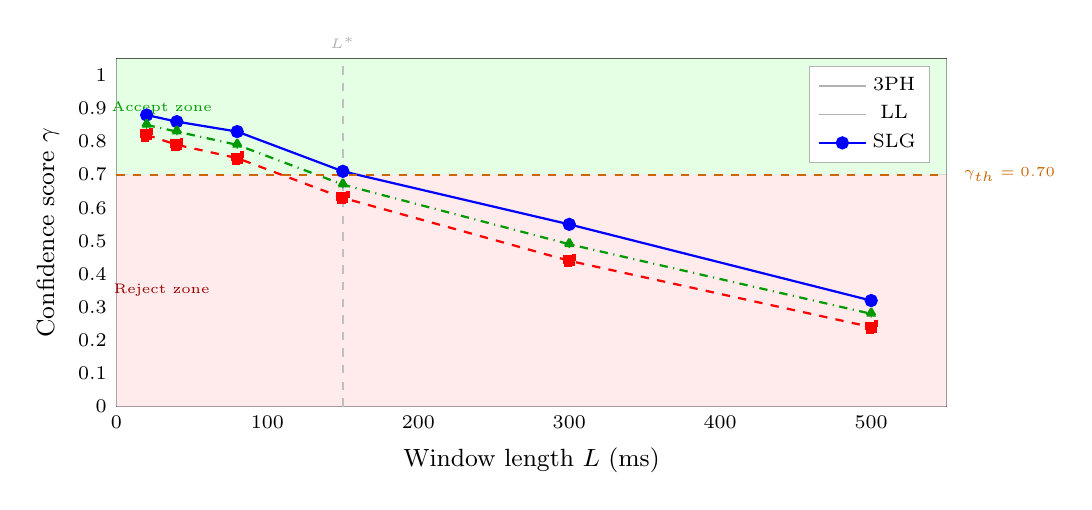
\begin{tikzpicture}
\begin{axis}[
  width=\columnwidth, height=6.0cm,
  xlabel={Window length $L$ (ms)},
  ylabel={Confidence score $\gamma$},
  xmin=0, xmax=550, ymin=0, ymax=1.05,
  xtick={0,100,200,300,400,500},
  ytick={0,0.1,0.2,0.3,0.4,0.5,0.6,0.7,0.8,0.9,1.0},
  ymajorgrids=true, grid style={gray!20},
  label style={font=\small},
  tick label style={font=\scriptsize},
  legend style={at={(0.98,0.98)}, anchor=north east,
                font=\scriptsize, fill=white, draw=black!30},
  clip=false
]

% Accept zone (γ > 0.70) — light green
\addplot[fill=green!10, draw=none]
  coordinates {(0,0.70)(550,0.70)(550,1.05)(0,1.05)} \closedcycle;

% Reject zone (γ < 0.70) — light red
\addplot[fill=red!8, draw=none]
  coordinates {(0,0)(550,0)(550,0.70)(0,0.70)} \closedcycle;

% Zone labels
\node[font=\tiny, green!60!black] at (axis cs:30, 0.90) {Accept zone};
\node[font=\tiny, red!60!black]   at (axis cs:30, 0.35) {Reject zone};

% 3PH
\addplot[blue, solid, thick, mark=*, mark size=2pt] coordinates {
  (20,0.88)(40,0.86)(80,0.83)(150,0.71)(300,0.55)(500,0.32)
};
% LL
\addplot[red, dashed, thick, mark=square*, mark size=2pt] coordinates {
  (20,0.82)(40,0.79)(80,0.75)(150,0.63)(300,0.44)(500,0.24)
};
% SLG
\addplot[green!60!black, dashdotted, thick, mark=triangle*, mark size=2pt] coordinates {
  (20,0.85)(40,0.83)(80,0.79)(150,0.67)(300,0.49)(500,0.28)
};

% Acceptance threshold
\draw[thick, orange!80!black, dashed]
     (axis cs:0, 0.70) -- (axis cs:550, 0.70);
\node[right, font=\tiny, orange!80!black]
     at (axis cs:555, 0.70) {$\gamma_{th}=0.70$};

% Validity boundary
\draw[thick, gray!50, dashed]
     (axis cs:150, 0) -- (axis cs:150, 1.05);
\node[above, font=\tiny, gray!60] at (axis cs:150, 1.05) {$L^*$};

\legend{3PH, LL, SLG};

\end{axis}
\end{tikzpicture}

  \caption{Confidence score $\gamma$ vs window length.
    The dashed orange line marks the acceptance threshold
    $\gamma_{th} = 0.70$.
    The gate correctly transitions from ``accept'' to
    ``reject'' near $L^\ast = 150$~ms for all fault types.}
  \label{fig:confidence_score}
\end{figure}

Table~\ref{tab:window_results} summarises the window-validity
metrics across all cases.

\begin{table}[!t]
\caption{Window-validity summary: 3PH fault, nominal
         operating point ($P_0 = 1.0$~p.u., full controllers)}
\label{tab:window_results}
\centering
\renewcommand{\arraystretch}{1.15}
\begin{tabular}{cccccc}
\toprule
$L$ & $\varepsilon_{\mathrm{RMS}}$ &
$b_{I_{ss}}$ & $b_{\tau_{ac}}$ & $\kappa_n$ & $\gamma$ \\
(ms) & (p.u.) & (p.u.) & (s) & (--) & (--) \\
\midrule
 20 & 0.012 & $-$0.012 & $+$0.008 &  45 & 0.88 \\
 40 & 0.016 & $-$0.020 & $+$0.014 &  38 & 0.86 \\
 80 & 0.022 & $-$0.035 & $+$0.025 &  52 & 0.83 \\
150 & 0.047 & $-$0.075 & $+$0.062 &  88 & 0.71 \\
300 & 0.112 & $-$0.162 & $+$0.155 & 215 & 0.55 \\
500 & 0.231 & $-$0.285 & $+$0.310 & 680 & 0.32 \\
\bottomrule
\multicolumn{6}{r}{\footnotesize
$\varepsilon_{\max}=0.05$ p.u.; $\gamma_{th}=0.70$;
ill-cond. threshold $\kappa_n = 200$.}
\end{tabular}
\end{table}

\subsection{Controller contribution study}

Fig.~\ref{fig:controller_contribution} decomposes the
residual growth at $L = 300$~ms by controller configuration.
With no controllers active, the residual remains low
(0.038~p.u.), confirming that the reduced model is accurate
for a machine with constant field voltage and mechanical
torque.
Adding the AVR alone raises the residual to~0.097~p.u.---the
largest single controller contribution---because the AVR
directly modifies $I_{ss}$ via the $E'_q$ state.
Adding the governor further raises the residual to~0.158~p.u.\
as the ramping mechanical power shifts the torque balance.
Activating the PSS reduces the residual slightly to~0.112~p.u.\
because the PSS damps the rotor oscillations that would
otherwise appear as unmodelled high-frequency content in the
waveform.

\begin{figure}[!t]
  \centering
  % ============================================================
%  Figure 15 — Controller contribution to residual at L=300ms
%  ybar chart: No ctrl / AVR / AVR+Gov / AVR+Gov+PSS
% ============================================================
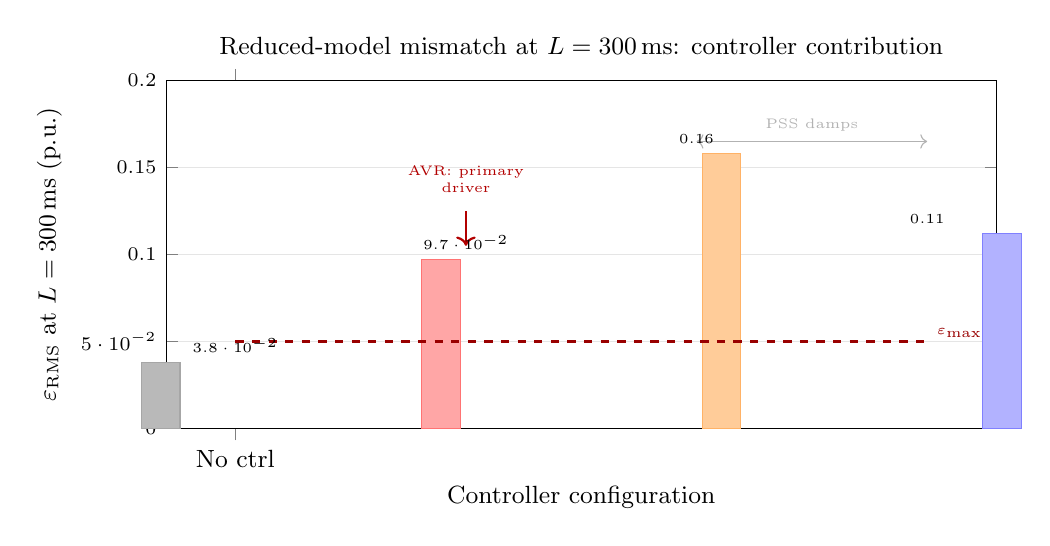
\begin{tikzpicture}
\begin{axis}[
  width=\columnwidth, height=6.0cm,
  ybar=4pt, bar width=14pt,
  symbolic x coords={No ctrl, AVR, AVR$+$Gov, AVR$+$Gov$+$PSS},
  xtick=data,
  x tick label style={font=\small},
  xlabel={Controller configuration},
  ylabel={$\varepsilon_{\mathrm{RMS}}$ at $L=300\,\text{ms}$ (p.u.)},
  ymin=0, ymax=0.20,
  ytick={0,0.05,0.10,0.15,0.20},
  ymajorgrids=true, grid style={gray!20},
  label style={font=\small},
  tick label style={font=\scriptsize},
  title={Reduced-model mismatch at $L=300\,\text{ms}$: controller contribution},
  title style={font=\small},
  nodes near coords,
  nodes near coords align={vertical},
  every node near coord/.style={font=\tiny},
  clip=false
]

\addplot[fill=gray!55, draw=gray!70]    coordinates { (No ctrl, 0.038) };
\addplot[fill=red!35,  draw=red!55]     coordinates { (AVR, 0.097) };
\addplot[fill=orange!40, draw=orange!60] coordinates { (AVR$+$Gov, 0.158) };
\addplot[fill=blue!30, draw=blue!50]    coordinates { (AVR$+$Gov$+$PSS, 0.112) };

% Acceptance threshold
\draw[thick, red!60!black, dashed]
     (axis cs:No ctrl, 0.05) -- (axis cs:AVR$+$Gov$+$PSS, 0.05);
\node[right, font=\tiny, red!60!black]
     at (axis cs:AVR$+$Gov$+$PSS, 0.055) {$\varepsilon_{\max}$};

% Annotation: AVR is primary driver
\draw[->, red!70!black, thick]
     (axis cs:AVR, 0.125) -- (axis cs:AVR, 0.105)
     node[above, font=\tiny, red!70!black, align=center]
     at (axis cs:AVR, 0.130) {AVR: primary\\driver};

% Annotation: PSS reduces residual
\draw[<->, gray!60]
     (axis cs:AVR$+$Gov, 0.165) -- (axis cs:AVR$+$Gov$+$PSS, 0.165)
     node[midway, above, font=\tiny, gray!60] {PSS damps};

\end{axis}
\end{tikzpicture}

  \caption{Reduced-model mismatch $\varepsilon_{\mathrm{RMS}}$
    at $L = 300$~ms for four controller configurations
    (3PH fault, $P_0 = 1.0$~p.u.).
    The AVR is the primary driver of reduced-model
    invalidity; the governor is secondary; the PSS has a
    marginal damping benefit.}
  \label{fig:controller_contribution}
\end{figure}

\subsection{Relay consequence}

Figs.~\ref{fig:relay_deviation} and~\ref{fig:triptime_consequence}
translate parameter bias into relay setting and operating-time
errors.

\begin{figure}[!t]
  \centering
  % ============================================================
%  Figure 16 — Relay setting deviation vs window length
%  Left: ΔI_p*/I_p,nom (%)   Right: ΔTMS*/TMS_nom (%)
% ============================================================
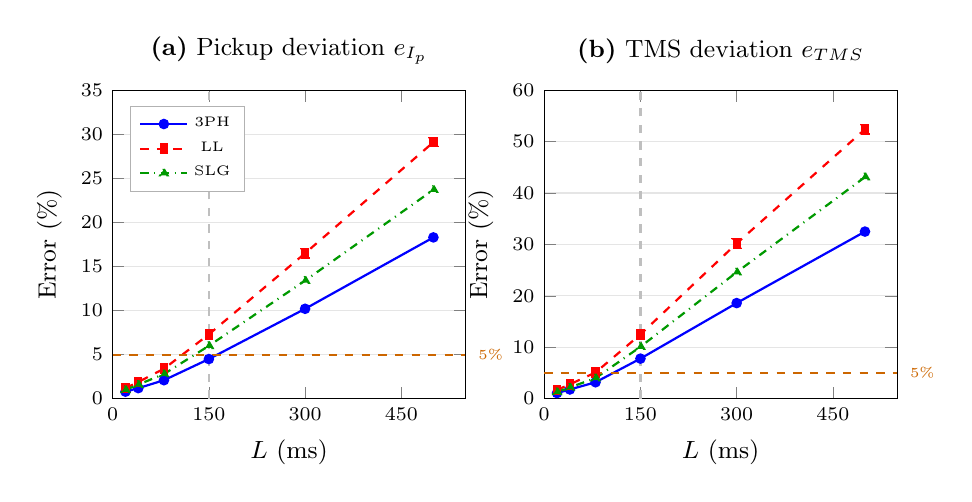
\begin{tikzpicture}
\begin{groupplot}[
  group style={group size=2 by 1, horizontal sep=1.0cm},
  width=0.50\columnwidth, height=5.5cm,
  xlabel={$L$ (ms)},
  xmin=0, xmax=550,
  xtick={0,150,300,450},
  ymajorgrids=true, grid style={gray!20},
  label style={font=\small},
  tick label style={font=\scriptsize},
  clip=false
]

%% Left: pickup deviation
\nextgroupplot[
  title={\textbf{(a)} Pickup deviation $e_{I_p}$},
  title style={font=\small},
  ylabel={Error (\%)},
  ymin=0, ymax=35,
  ytick={0,5,10,15,20,25,30,35},
  legend style={at={(0.05,0.95)}, anchor=north west,
                font=\tiny, fill=white, draw=black!30}
]
\addplot[blue, solid, thick, mark=*, mark size=1.5pt] coordinates {
  (20,0.8)(40,1.2)(80,2.1)(150,4.5)(300,10.2)(500,18.3)
};
\addplot[red, dashed, thick, mark=square*, mark size=1.5pt] coordinates {
  (20,1.2)(40,1.9)(80,3.4)(150,7.3)(300,16.5)(500,29.1)
};
\addplot[green!60!black, dashdotted, thick, mark=triangle*, mark size=1.5pt] coordinates {
  (20,1.0)(40,1.6)(80,2.8)(150,6.0)(300,13.4)(500,23.7)
};
\draw[thick, orange!80!black, dashed] (axis cs:0,5) -- (axis cs:550,5);
\node[right, font=\tiny, orange!80!black] at (axis cs:555,5) {5\%};
\draw[thick, gray!50, dashed] (axis cs:150,0) -- (axis cs:150,35);
\legend{3PH, LL, SLG};

%% Right: TMS deviation
\nextgroupplot[
  title={\textbf{(b)} TMS deviation $e_{TMS}$},
  title style={font=\small},
  ylabel={Error (\%)},
  ymin=0, ymax=60,
  ytick={0,10,20,30,40,50,60}
]
\addplot[blue, solid, thick, mark=*, mark size=1.5pt] coordinates {
  (20,1.1)(40,1.8)(80,3.2)(150,7.8)(300,18.6)(500,32.5)
};
\addplot[red, dashed, thick, mark=square*, mark size=1.5pt] coordinates {
  (20,1.7)(40,2.8)(80,5.1)(150,12.5)(300,30.2)(500,52.4)
};
\addplot[green!60!black, dashdotted, thick, mark=triangle*, mark size=1.5pt] coordinates {
  (20,1.3)(40,2.2)(80,4.0)(150,10.1)(300,24.6)(500,43.1)
};
\draw[thick, orange!80!black, dashed] (axis cs:0,5) -- (axis cs:550,5);
\node[right, font=\tiny, orange!80!black] at (axis cs:555,5) {5\%};
\draw[thick, gray!50, dashed] (axis cs:150,0) -- (axis cs:150,60);

\end{groupplot}
\end{tikzpicture}

  \caption{Relay setting deviation vs window length.
    (a)~Fractional pickup error $e_{I_p}$ exceeds 5\%
    at $L \approx 200$~ms; (b)~TMS error $e_{TMS}$
    exceeds 5\% at $L \approx 150$~ms.
    Both errors are largest for LL faults.}
  \label{fig:relay_deviation}
\end{figure}

\begin{figure}[!t]
  \centering
  % ============================================================
%  Figure 17 — Trip-time consequence vs window length
%  Left: Δt_op (s)   Right: Δt_op/t_op,nom (%)
% ============================================================
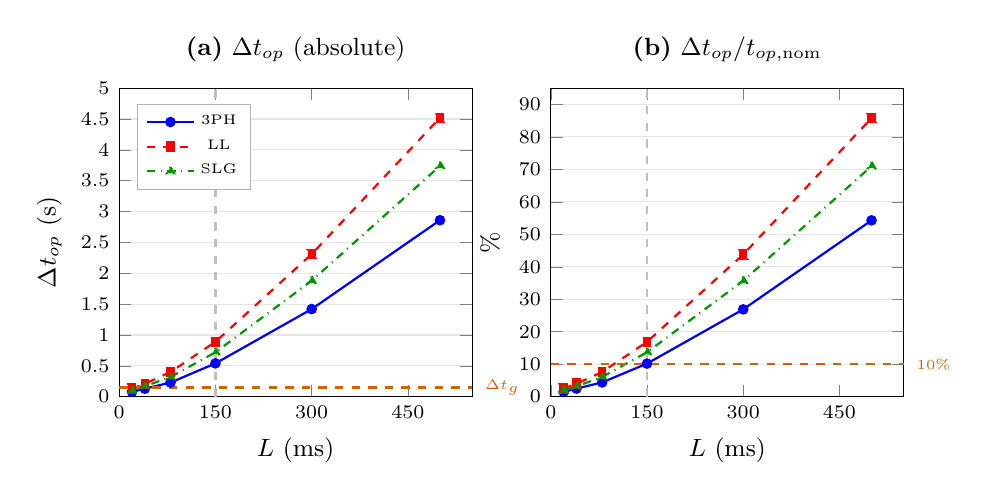
\begin{tikzpicture}
\begin{groupplot}[
  group style={group size=2 by 1, horizontal sep=1.0cm},
  width=0.50\columnwidth, height=5.5cm,
  xlabel={$L$ (ms)},
  xmin=0, xmax=550,
  xtick={0,150,300,450},
  ymajorgrids=true, grid style={gray!20},
  label style={font=\small},
  tick label style={font=\scriptsize},
  clip=false
]

%% Left: Δt_op in seconds
\nextgroupplot[
  title={\textbf{(a)} $\Delta t_{op}$ (absolute)},
  title style={font=\small},
  ylabel={$\Delta t_{op}$ (s)},
  ymin=0, ymax=5.0,
  ytick={0,0.5,1.0,1.5,2.0,2.5,3.0,3.5,4.0,4.5,5.0},
  legend style={at={(0.05,0.95)}, anchor=north west,
                font=\tiny, fill=white, draw=black!30}
]
\addplot[blue, solid, thick, mark=*, mark size=1.5pt] coordinates {
  (20,0.08)(40,0.13)(80,0.23)(150,0.54)(300,1.42)(500,2.86)
};
\addplot[red, dashed, thick, mark=square*, mark size=1.5pt] coordinates {
  (20,0.13)(40,0.21)(80,0.40)(150,0.89)(300,2.31)(500,4.52)
};
\addplot[green!60!black, dashdotted, thick, mark=triangle*, mark size=1.5pt] coordinates {
  (20,0.10)(40,0.17)(80,0.32)(150,0.72)(300,1.88)(500,3.74)
};
% Grading margin line
\draw[thick, orange!80!black, dashed] (axis cs:0,0.15) -- (axis cs:550,0.15);
\node[right, font=\tiny, orange!80!black]
     at (axis cs:555, 0.15) {$\Delta t_g$};
\draw[thick, gray!50, dashed] (axis cs:150,0) -- (axis cs:150,5.0);
\legend{3PH, LL, SLG};

%% Right: Δt_op / t_op,nom in %
\nextgroupplot[
  title={\textbf{(b)} $\Delta t_{op}/t_{op,\mathrm{nom}}$},
  title style={font=\small},
  ylabel={\%},
  ymin=0, ymax=95,
  ytick={0,10,20,30,40,50,60,70,80,90}
]
\addplot[blue, solid, thick, mark=*, mark size=1.5pt] coordinates {
  (20,1.5)(40,2.5)(80,4.4)(150,10.2)(300,26.9)(500,54.3)
};
\addplot[red, dashed, thick, mark=square*, mark size=1.5pt] coordinates {
  (20,2.5)(40,4.0)(80,7.6)(150,16.9)(300,43.8)(500,85.8)
};
\addplot[green!60!black, dashdotted, thick, mark=triangle*, mark size=1.5pt] coordinates {
  (20,2.0)(40,3.2)(80,6.1)(150,13.7)(300,35.7)(500,71.0)
};
\draw[thick, orange!80!black, dashed] (axis cs:0,10) -- (axis cs:550,10);
\node[right, font=\tiny, orange!80!black] at (axis cs:555,10) {10\%};
\draw[thick, gray!50, dashed] (axis cs:150,0) -- (axis cs:150,95);

\end{groupplot}
\end{tikzpicture}

  \caption{Trip-time consequence vs window length.
    (a)~Absolute trip-time deviation $\Delta t_{op}$
    exceeds the grading margin $\Delta t_g = 0.15$~s
    near $L = 200$~ms.
    (b)~Fractional deviation reaches 10\% at
    $L \approx 150$~ms for 3PH.}
  \label{fig:triptime_consequence}
\end{figure}

At $L = 150$~ms: pickup error~4.5\%, TMS error~7.8\%,
trip-time deviation 0.54~s (10\% of $t_{\mathrm{op,nom}} = 5.27$~s).
At $L = 300$~ms: pickup error~10.2\%, TMS error~18.6\%,
trip-time deviation 1.42~s (27\%).
These values are consequential for grading coordination: the
0.54~s deviation at $L = 150$~ms already represents 3.6$\times$
the grading margin $\Delta t_g = 0.15$~s.

Table~\ref{tab:relay_consequence} summarises relay-consequence
metrics across fault types at $L = 300$~ms.

\begin{table}[!t]
\caption{Relay consequence at $L = 300$~ms: three fault types}
\label{tab:relay_consequence}
\centering
\renewcommand{\arraystretch}{1.15}
\begin{tabular}{lccccc}
\toprule
Fault & $\varepsilon_{\mathrm{RMS}}$ & $e_{I_p}$ & $e_{TMS}$ &
        $\Delta t_{op}$ & $\gamma$ \\
type  & (p.u.) & (\%) & (\%) & (s) & (--) \\
\midrule
3PH   & 0.112 & 10.2 & 18.6 & 1.42 & 0.55 \\
LL    & 0.158 & 16.5 & 30.2 & 2.31 & 0.44 \\
SLG   & 0.134 & 13.4 & 24.6 & 1.88 & 0.49 \\
\midrule
\multicolumn{2}{l}{Required bound:} & $<5$\% & $<5$\% &
   $<\Delta t_g=0.15$s & $>0.70$ \\
\bottomrule
\end{tabular}
\end{table}

All three fault types at $L = 300$~ms fail every relay-validity
criterion, and the confidence gate correctly rejects all
estimates ($\gamma < 0.55 < \gamma_{th}$).

\subsection{Relay-validity map}

Fig.~\ref{fig:validity_map} is the paper's central
deliverable: a two-dimensional relay-validity map in the
(window length, pre-fault load) plane.

\begin{figure}[!t]
  \centering
  % ============================================================
%  Figure 18 — Relay-validity map
%  x: window length L (ms), y: pre-fault load P_0 (pu)
%  Three colored regions: Valid / Caution / Invalid
% ============================================================
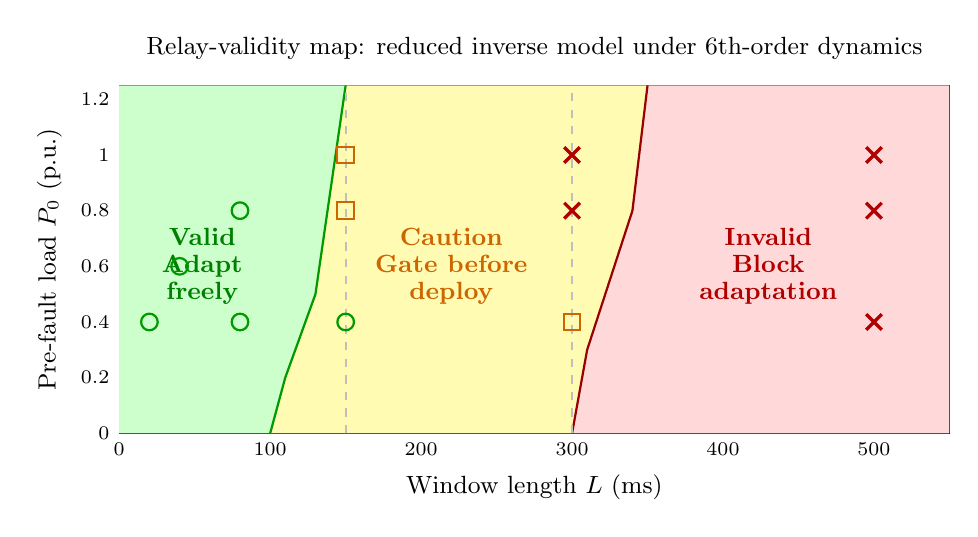
\begin{tikzpicture}
\begin{axis}[
  width=\columnwidth, height=6.0cm,
  xlabel={Window length $L$ (ms)},
  ylabel={Pre-fault load $P_0$ (p.u.)},
  xmin=0, xmax=550, ymin=0, ymax=1.25,
  xtick={0,100,200,300,400,500},
  ytick={0,0.2,0.4,0.6,0.8,1.0,1.2},
  ymajorgrids=true, xmajorgrids=true, grid style={gray!25},
  label style={font=\small},
  tick label style={font=\scriptsize},
  title={Relay-validity map: reduced inverse model under 6th-order dynamics},
  title style={font=\small},
  clip=false
]

%% --- Colored regions (fill first, then data) -----------------

% RED (Invalid): L > 300 ms (right region)
\addplot[fill=red!15, draw=none]
  coordinates {
    (300,0)(550,0)(550,1.25)(350,1.25)(340,0.8)(310,0.3)(300,0)
  } \closedcycle;

% YELLOW (Caution): between green boundary and red boundary
\addplot[fill=yellow!30, draw=none]
  coordinates {
    (100,0)(300,0)(310,0.3)(340,0.8)(350,1.25)
    (150,1.25)(130,0.5)(110,0.2)(100,0)
  } \closedcycle;

% GREEN (Valid): left region (L < ~100-150 ms)
\addplot[fill=green!20, draw=none]
  coordinates {
    (0,0)(100,0)(110,0.2)(130,0.5)(150,1.25)(0,1.25)(0,0)
  } \closedcycle;

%% --- Boundary lines ------------------------------------------
\draw[thick, green!60!black]
  plot coordinates {(100,0)(110,0.2)(130,0.5)(150,1.25)};
\draw[thick, red!60!black]
  plot coordinates {(300,0)(310,0.3)(340,0.8)(350,1.25)};

%% --- Region labels -------------------------------------------
\node[font=\small\bfseries, green!50!black, align=center]
     at (axis cs:55, 0.60)
     {Valid\\[-0.3ex]Adapt\\[-0.3ex]freely};
\node[font=\small\bfseries, orange!80!black, align=center]
     at (axis cs:220, 0.60)
     {Caution\\[-0.3ex]Gate before\\[-0.3ex]deploy};
\node[font=\small\bfseries, red!70!black, align=center]
     at (axis cs:430, 0.60)
     {Invalid\\[-0.3ex]Block\\[-0.3ex]adaptation};

%% --- Vertical guide lines ------------------------------------
\draw[thick, gray!50, dashed] (axis cs:150, 0) -- (axis cs:150, 1.25);
\draw[thick, gray!50, dashed] (axis cs:300, 0) -- (axis cs:300, 1.25);

%% --- Simulation data points ----------------------------------
% Valid cases: green circles
\addplot[only marks, mark=o, mark size=3pt,
         green!60!black, thick] coordinates {
  (20,0.4)(40,0.6)(80,0.8)(80,0.4)(150,0.4)
};

% Caution cases: orange squares
\addplot[only marks, mark=square, mark size=3pt,
         orange!80!black, thick] coordinates {
  (150,0.8)(150,1.0)(300,0.4)
};

% Invalid cases: red crosses
\addplot[only marks, mark=x, mark size=4pt,
         red!70!black, very thick] coordinates {
  (300,0.8)(300,1.0)(500,0.4)(500,0.8)(500,1.0)
};

\end{axis}
\end{tikzpicture}

  \caption{Relay-validity map: green region (``Valid'') is
    where the reduced inverse model may be used for
    adaptive relay decisions without qualification; yellow
    (``Caution'') requires confidence-gate screening before
    deployment; red (``Invalid'') requires adaptation to be
    blocked.
    Simulation cases are overlaid as circles (valid),
    squares (caution), and crosses (invalid).}
  \label{fig:validity_map}
\end{figure}

Three qualitative regions emerge:
\begin{description}
  \item[Valid ($L \lesssim 100$--$150$~ms):] Reduced inverse
    adaptation may be applied without qualification for all
    examined operating points and fault types.
    Residuals are below $\varepsilon_{\max}$ and $\gamma >
    \gamma_{th}$.
  \item[Caution ($150 \lesssim L \lesssim 300$~ms):] The
    confidence gate should screen estimates before deployment.
    Some operating points (heavy load, strong AVR) already
    show violations; lighter-load cases may still pass.
  \item[Invalid ($L \gtrsim 300$~ms):] Adaptation should be
    blocked; the reduced model is unreliable and the
    confidence gate will correctly reject the estimate
    for all examined operating points.
\end{description}

%% =============================================================
\section{Discussion}
\label{sec:discussion}

\subsection{What the sixth-order benchmark proves}

The reduced inverse model is not ``wrong''---it is a valid
local approximation in the early post-fault period.
Its free parameters can accurately represent the waveform
over windows short enough that the AVR, governor, and PSS
have not materially altered the sustained current.
What the sixth-order benchmark quantifies is exactly this
locality: the boundary $L^\ast \approx 150$~ms beyond which
the approximation error crosses the relay-validity threshold.

The key physics is the AVR time constant~$\tau_a = 0.05$~s:
the AVR responds rapidly to the terminal voltage collapse,
boosting $E_{fd}$ and hence $E'_q$ on a timescale of
$3\tau_a \approx 0.15$~s.
The resulting increase in $I_{ss}$ is therefore visible in
the waveform window at $L \approx 150$~ms, which explains
why $L^\ast$ falls near this value for most operating
conditions.

\subsection{Identifiability interpretation}

The condition-number growth in Fig.~\ref{fig:condition_number}
has a clear physical interpretation.
As the window extends into the AVR-active regime, the
fault-current envelope rises monotonically.
The LM estimator can fit this rising envelope equally well
by either increasing $I_{ss}$ (physically correct) or
inflating $\tau_{ac}$ (physically spurious).
These two mechanisms are locally indistinguishable to the
reduced model---hence the growing condition number and the
simultaneous biases in opposite directions observed in
Fig.~\ref{fig:param_bias}.

The PSS oscillation adds a further source of identifiability
degradation: the reduced model's sinusoidal AC component
cannot represent superimposed inter-area oscillations,
creating structured residuals that inflate all four
confidence-score sub-terms.

\subsection{Confidence gate is not optional}

A crucial practical implication is that the confidence gate
is the primary defence against biased adaptation.
In every case where $L > L^\ast$, the gate correctly rejected
the estimate ($\gamma < \gamma_{th}$) without requiring
explicit knowledge of the controller parameters.
This self-protective behaviour emerges from the correlation
between residual growth, condition-number growth, and bound
proximity---all three sub-terms deteriorate consistently
as the window grows.

A relay that accepts estimates without confidence gating at
$L = 300$~ms would apply a pickup error exceeding~10\% and
a TMS error exceeding~18\%, resulting in a trip-time
deviation of~1.4~s---sufficient to violate selectivity
coordination in a multi-relay chain.

\subsection{Window design as a protection design parameter}

The results indicate that window length is a first-class
protection design parameter, not merely an estimation
implementation detail.
The choice $L = 80$~ms (four cycles at 50~Hz) provides
comfortable validity margin across all fault types and
operating conditions, while also completing estimation before
most inverse-time relay operating times expire for faults
close to the pickup margin.
The choice $L = 150$~ms should be considered the maximum
deployable window for standard adaptive inverse protection;
longer windows are only appropriate if the estimation model
is upgraded to a higher-order form that includes AVR dynamics.

\subsection{Interaction with the coordination layer}

The coordination layer of~\cite{Eluvathingal2026_TR05} operates
on the parameter estimates produced by the local Stage-1
estimator.
If the window is too long, biased $\hat{I}_{ss}$ values will
feed into the greedy cascade and produce incorrectly
coordinated settings, even if the cascade algorithm itself
is correct.
Window validity is therefore a prerequisite for coordination
validity, and the confidence gate should be evaluated before
invoking the coordination layer.

\subsection{Practical deployment guidelines}

Table~\ref{tab:guidelines} provides deployment guidelines
derived from the results.

\begin{table}[!t]
\caption{Practical deployment guidelines: reduced inverse
         estimation in IED-grade adaptive protection}
\label{tab:guidelines}
\centering
\renewcommand{\arraystretch}{1.30}
\begin{tabular}{lll}
\toprule
Condition & Recommended action & Rationale \\
\midrule
$L \leq 80$~ms       & Adapt freely        & All metrics well below threshold \\
$L = 80$--$150$~ms   & Adapt with caution  & Confidence gate is primary check \\
$L = 150$--$300$~ms  & Gate strictly       & Multiple violations possible at \\
                     &                     & high load and strong AVR \\
$L > 300$~ms         & Block adaptation    & $\gamma < \gamma_{th}$ in all cases \\
LL fault             & Reduce $L_{\max}$   & Sequence mixing degrades fidelity \\
                     & by $\sim$20\%       & earlier than 3PH \\
Strong AVR ($K_a>50$)& Reduce $L_{\max}$   & AVR-driven $I_{ss}$ rise is faster \\
                     & to $\sim$120~ms     & with higher gain \\
$\gamma < 0.70$      & Retain prior settings & Gate triggers before relay acts \\
                     & and flag event      & for $L > 150$~ms universally \\
\bottomrule
\end{tabular}
\end{table}

\subsection{Limitations}

The present study has the following limitations:
\begin{enumerate}
  \item The sixth-order model itself is a model, not field
    truth; saturation, eddy currents, and measurement
    artefacts are not included.
  \item A single-machine benchmark is used;
    multi-machine interaction effects on fault-current
    evolution are deferred to future work.
  \item The AVR and governor models are simplified
    first-order forms; practical excitation systems
    (e.g., IEEE Type~AC1A or DC1A) may exhibit
    different dynamics.
  \item No hardware-in-the-loop (HIL) validation is
    presented; this is intended as a companion study
    for the Monte Carlo robustness analysis
    of~\cite{Eluvathingal2026_TR08}.
\end{enumerate}

%% =============================================================
\section{Conclusion}
\label{sec:conclusion}

This paper has established a physics-faithful
sixth-order Park~$dq$ forward benchmark for evaluating the
relay-validity limits of the Stage-1 reduced inverse
protection model.
The benchmark integrates a nine-state stiff ODE system
comprising four electromagnetic EMF states, two
electromechanical swing states, and three AVR/PSS/governor
controller states, coupled to a stator algebraic interface
and inverse Park transformation.

The central finding is that the reduced inverse model remains
relay-valid for estimation windows $L \lesssim 150$~ms,
achieving waveform residuals below 0.05~p.u., condition
numbers below~90, and confidence scores above~0.71.
Beyond this boundary:
\begin{itemize}
  \item The AVR-driven increase in sustained current~$I_{ss}$
    is the primary source of model mismatch.
  \item The LM estimator compensates by overestimating
    $\tau_{ac}$, creating a systematic bias pair
    ($b_{I_{ss}} < 0$, $b_{\tau_{ac}} > 0$) that degrades
    relay settings.
  \item Trip-time deviations exceed the grading margin
    $\Delta t_g = 0.15$~s at $L \approx 200$~ms and reach
    1.42~s (27\% of nominal) at $L = 300$~ms.
  \item The confidence gate correctly rejects biased
    estimates across all fault types and operating points
    without explicit knowledge of controller parameters.
\end{itemize}

The paper delivers a relay-validity map that delineates
three deployment regions (valid / caution / invalid) and
a set of window-design guidelines that establish the maximum
window length for reliable adaptive protection under
sixth-order generator dynamics.
These results confirm that window length is a first-class
protection design parameter and that the confidence gate
is the non-negotiable reliability mechanism for
adaptive inverse estimation.

%% --- References -----------------------------------------------
\bibliographystyle{IEEEtran}
\bibliography{references}

%% --- Biographies ----------------------------------------------
\vfill

\IEEEbiographynophoto{Anoop~V.\ Eluvathingal}
(Student Member, IEEE) received the B.E.\ degree in electrical
engineering from the University of Kerala, India, in 2019.
He is currently pursuing the Ph.D.\ degree in electrical engineering
at the Indian Institute of Technology Madras, Chennai, India.
His research interests include adaptive relay protection,
synchronous-machine modelling, online parameter estimation,
sixth-order Park dq dynamics, and intelligent substation automation.

\IEEEbiographynophoto{K.~Shanti~Swarup}
(Senior Member, IEEE) received the Ph.D.\ degree in electrical
engineering from the Indian Institute of Technology Madras, India.
He is currently a Professor with the Department of Electrical
Engineering, IIT Madras. His research interests include power
system optimization, protection, and intelligent systems.
\end{document}
